% Generated by 02_Code/build_latex_package.py. Paths are relative to package root.

\subsection{Pickup and dropoff demand maps}

\begin{figure}[p]\centering
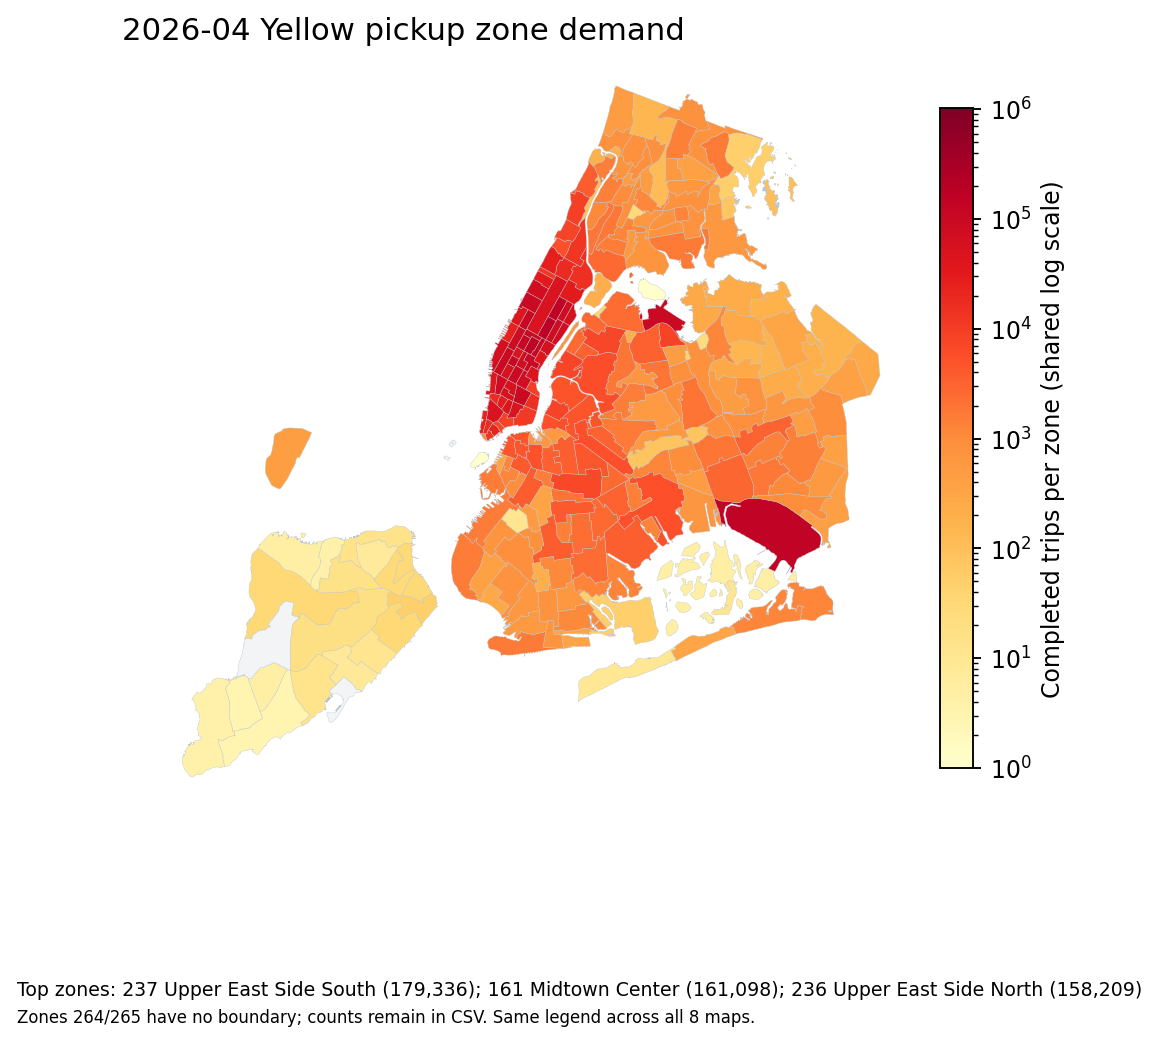
\includegraphics[width=.83\textwidth,height=.72\textheight,keepaspectratio]{04_Results/Task_2/figures/hotspot_2026-04_yellow_pickup.png}
\caption{2026-04 Yellow Taxi pickup counts by TLC zone. The color shows completed trip records, not people or all requests. Zones 264 and 265 have no polygon; their counts remain in the CSV.}\label{fig:hot04yPU}
\end{figure}

\begin{figure}[p]\centering
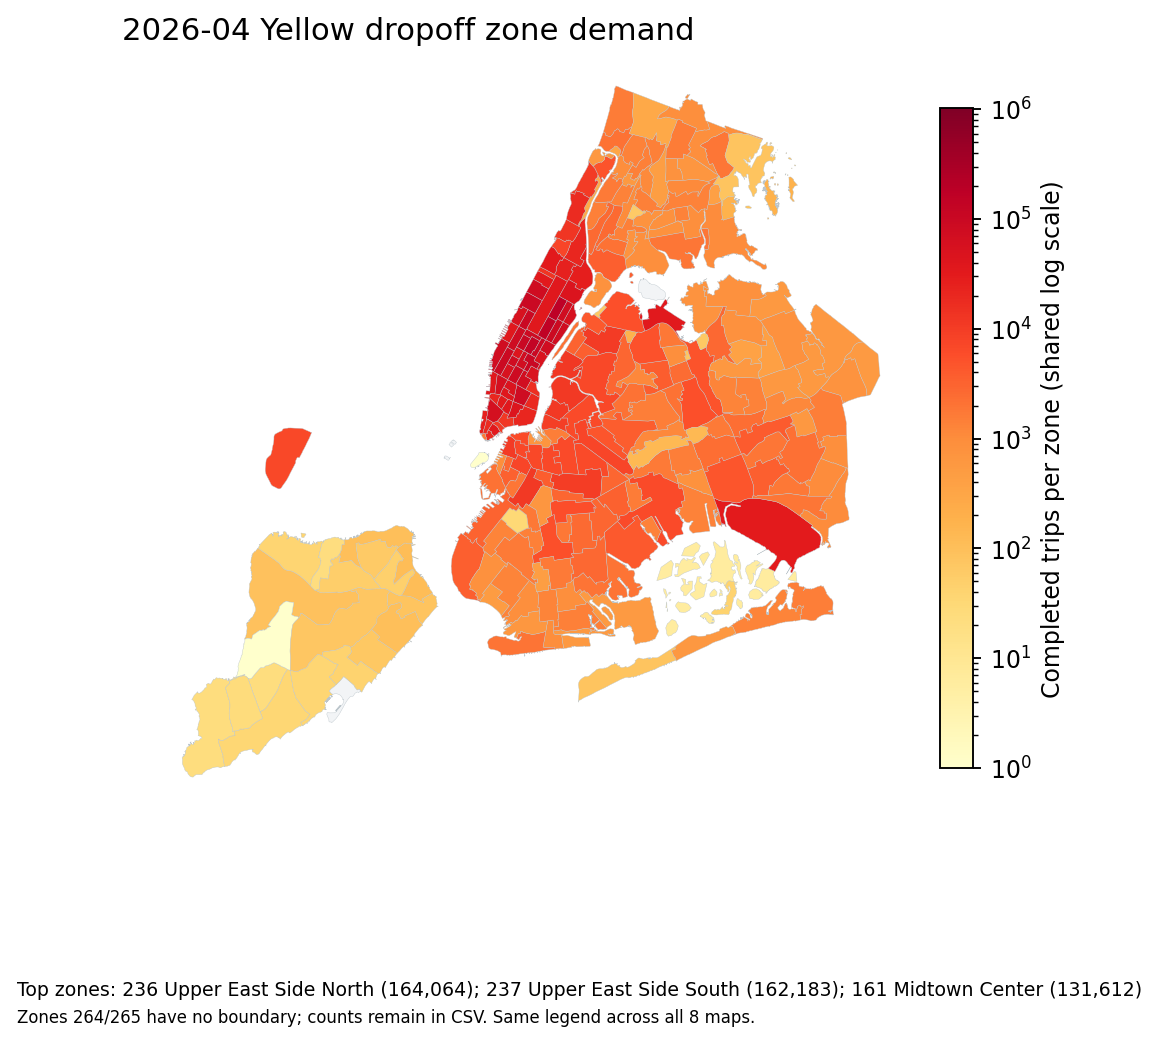
\includegraphics[width=.83\textwidth,height=.72\textheight,keepaspectratio]{04_Results/Task_2/figures/hotspot_2026-04_yellow_dropoff.png}
\caption{2026-04 Yellow Taxi dropoff counts by TLC zone. The color shows completed trip records, not people or all requests. Zones 264 and 265 have no polygon; their counts remain in the CSV.}\label{fig:hot04yDO}
\end{figure}

\begin{figure}[p]\centering
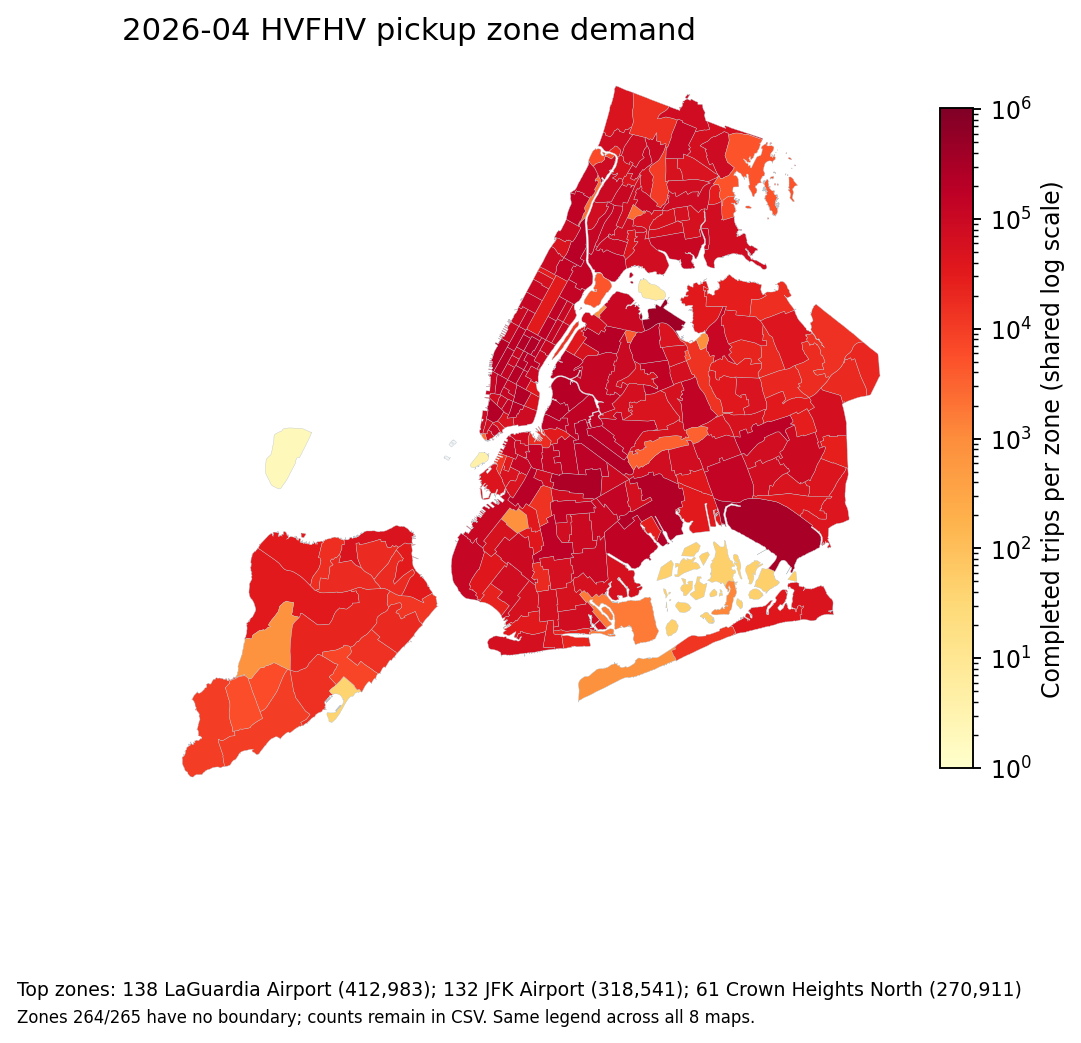
\includegraphics[width=.83\textwidth,height=.72\textheight,keepaspectratio]{04_Results/Task_2/figures/hotspot_2026-04_hvfhv_pickup.png}
\caption{2026-04 HVFHV pickup counts by TLC zone. The color shows completed trip records, not people or all requests. Zones 264 and 265 have no polygon; their counts remain in the CSV.}\label{fig:hot04hPU}
\end{figure}

\begin{figure}[p]\centering
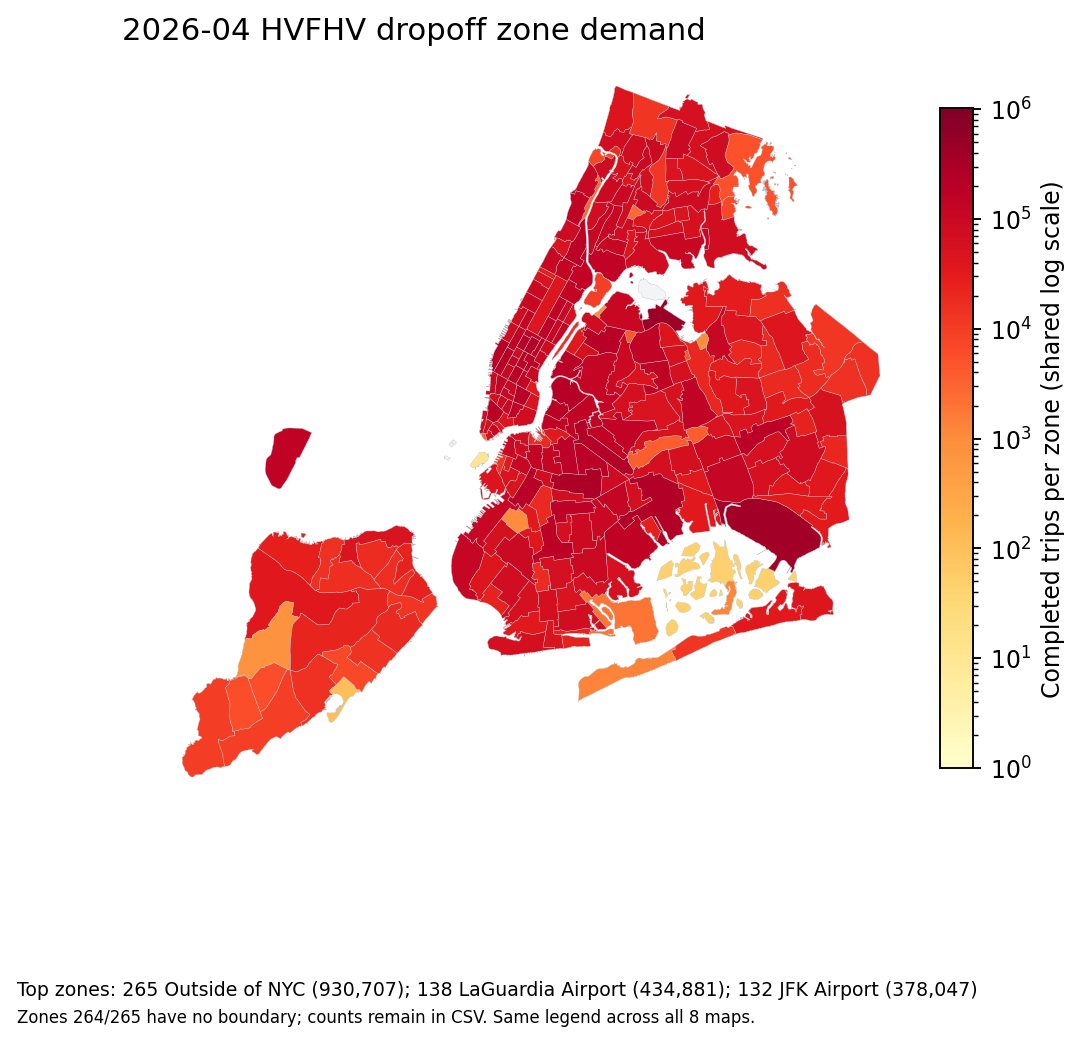
\includegraphics[width=.83\textwidth,height=.72\textheight,keepaspectratio]{04_Results/Task_2/figures/hotspot_2026-04_hvfhv_dropoff.png}
\caption{2026-04 HVFHV dropoff counts by TLC zone. The color shows completed trip records, not people or all requests. Zones 264 and 265 have no polygon; their counts remain in the CSV.}\label{fig:hot04hDO}
\end{figure}

\begin{figure}[p]\centering
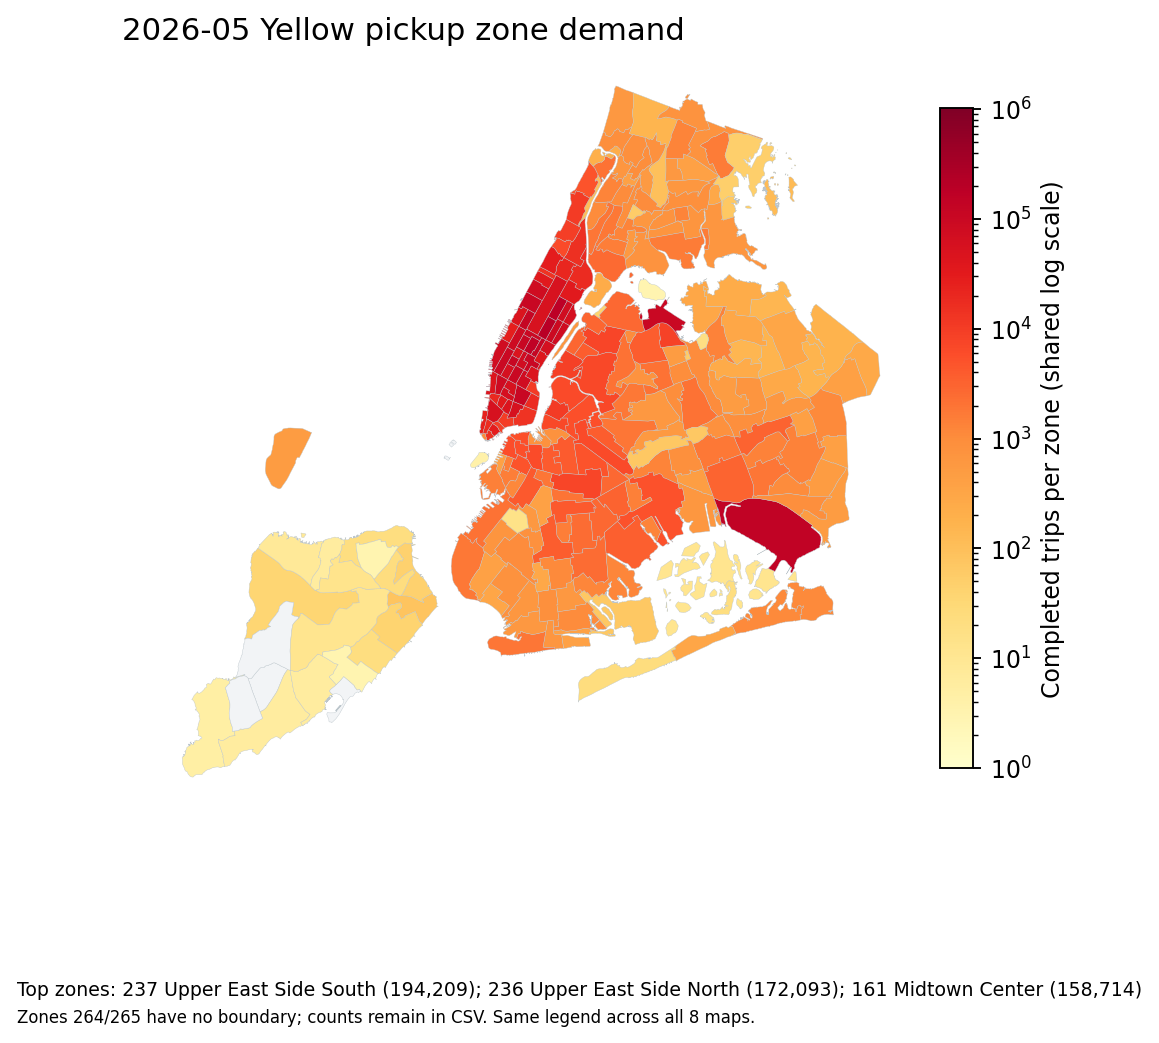
\includegraphics[width=.83\textwidth,height=.72\textheight,keepaspectratio]{04_Results/Task_2/figures/hotspot_2026-05_yellow_pickup.png}
\caption{2026-05 Yellow Taxi pickup counts by TLC zone. The color shows completed trip records, not people or all requests. Zones 264 and 265 have no polygon; their counts remain in the CSV.}\label{fig:hot05yPU}
\end{figure}

\begin{figure}[p]\centering
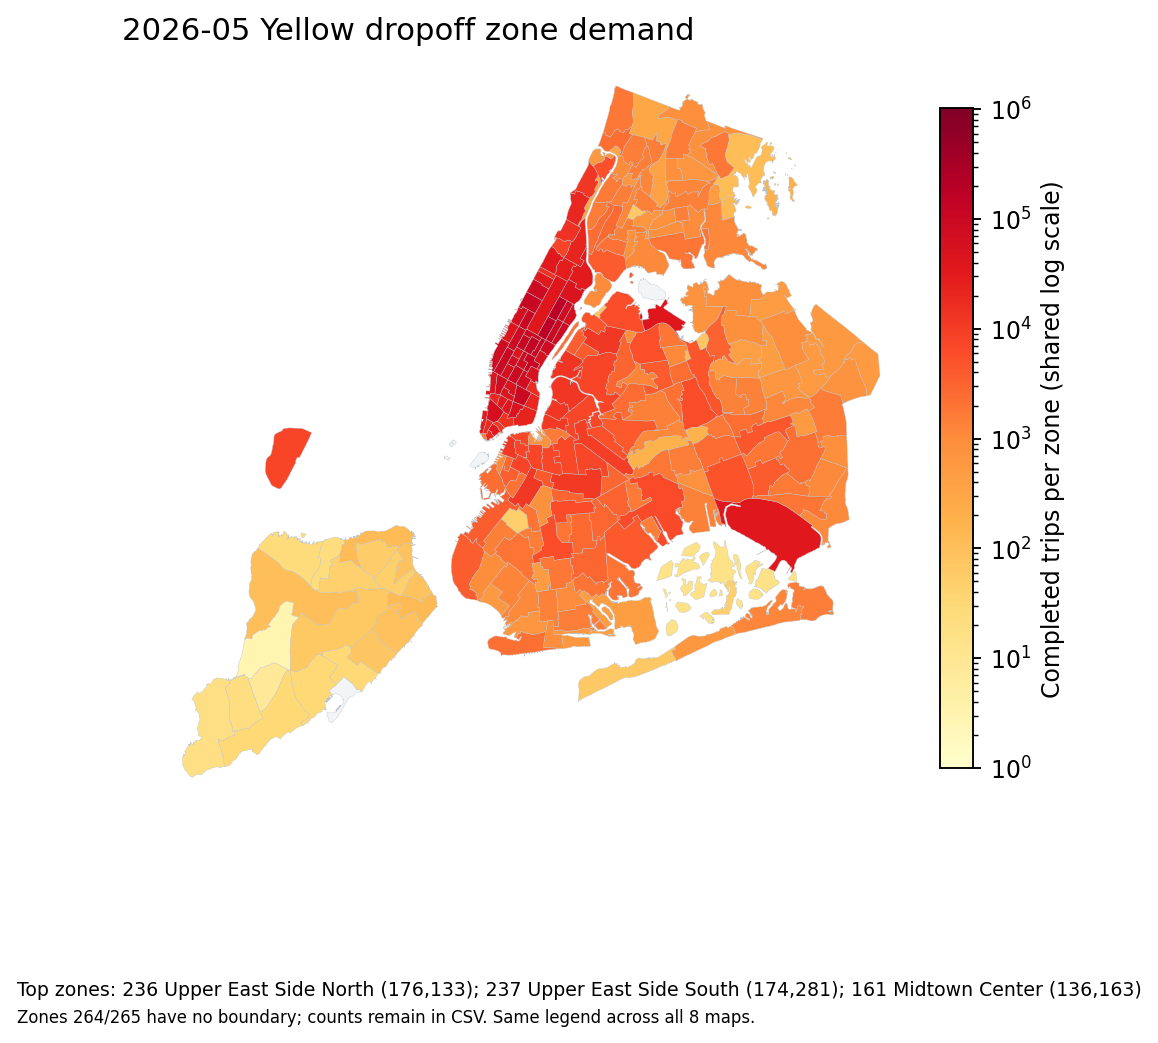
\includegraphics[width=.83\textwidth,height=.72\textheight,keepaspectratio]{04_Results/Task_2/figures/hotspot_2026-05_yellow_dropoff.png}
\caption{2026-05 Yellow Taxi dropoff counts by TLC zone. The color shows completed trip records, not people or all requests. Zones 264 and 265 have no polygon; their counts remain in the CSV.}\label{fig:hot05yDO}
\end{figure}

\begin{figure}[p]\centering
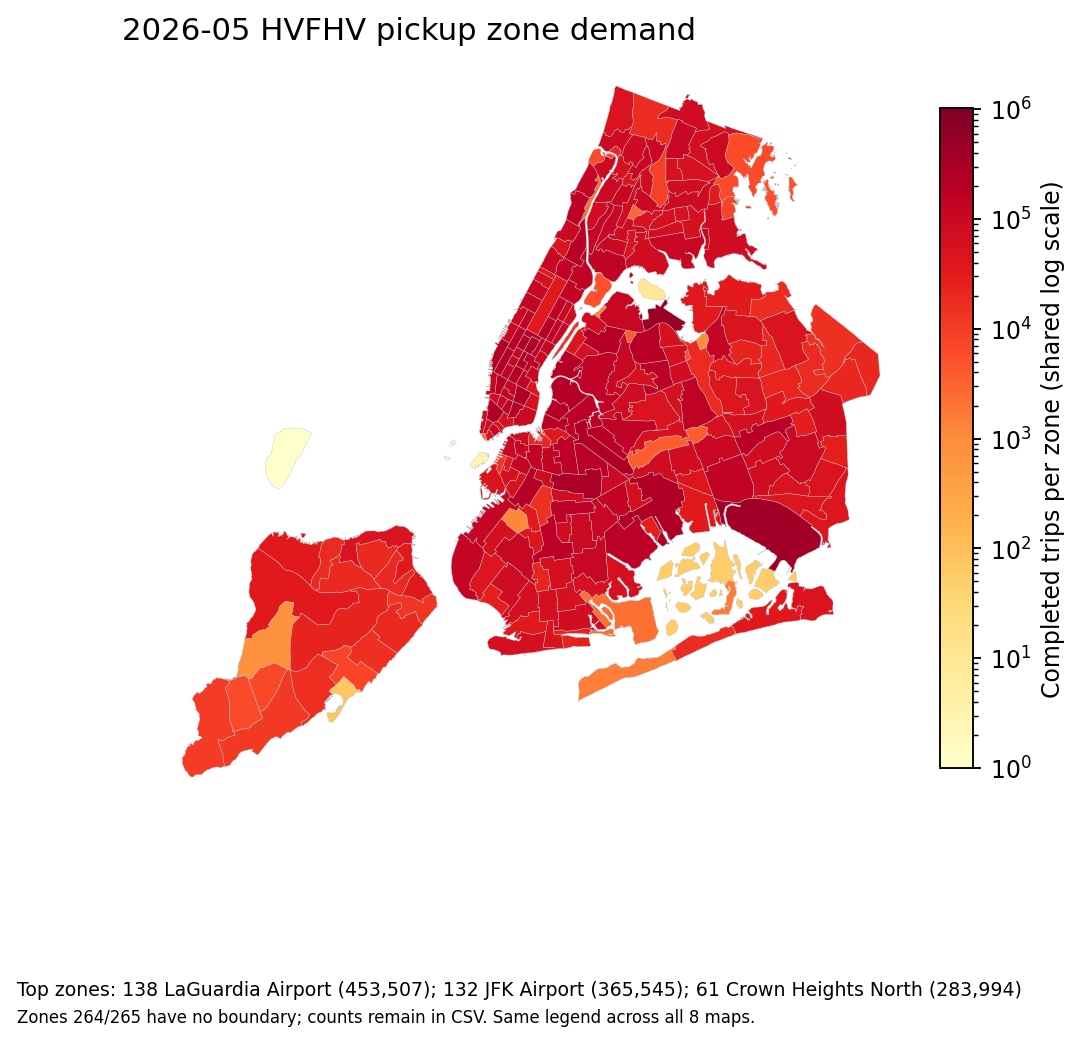
\includegraphics[width=.83\textwidth,height=.72\textheight,keepaspectratio]{04_Results/Task_2/figures/hotspot_2026-05_hvfhv_pickup.png}
\caption{2026-05 HVFHV pickup counts by TLC zone. The color shows completed trip records, not people or all requests. Zones 264 and 265 have no polygon; their counts remain in the CSV.}\label{fig:hot05hPU}
\end{figure}

\begin{figure}[p]\centering
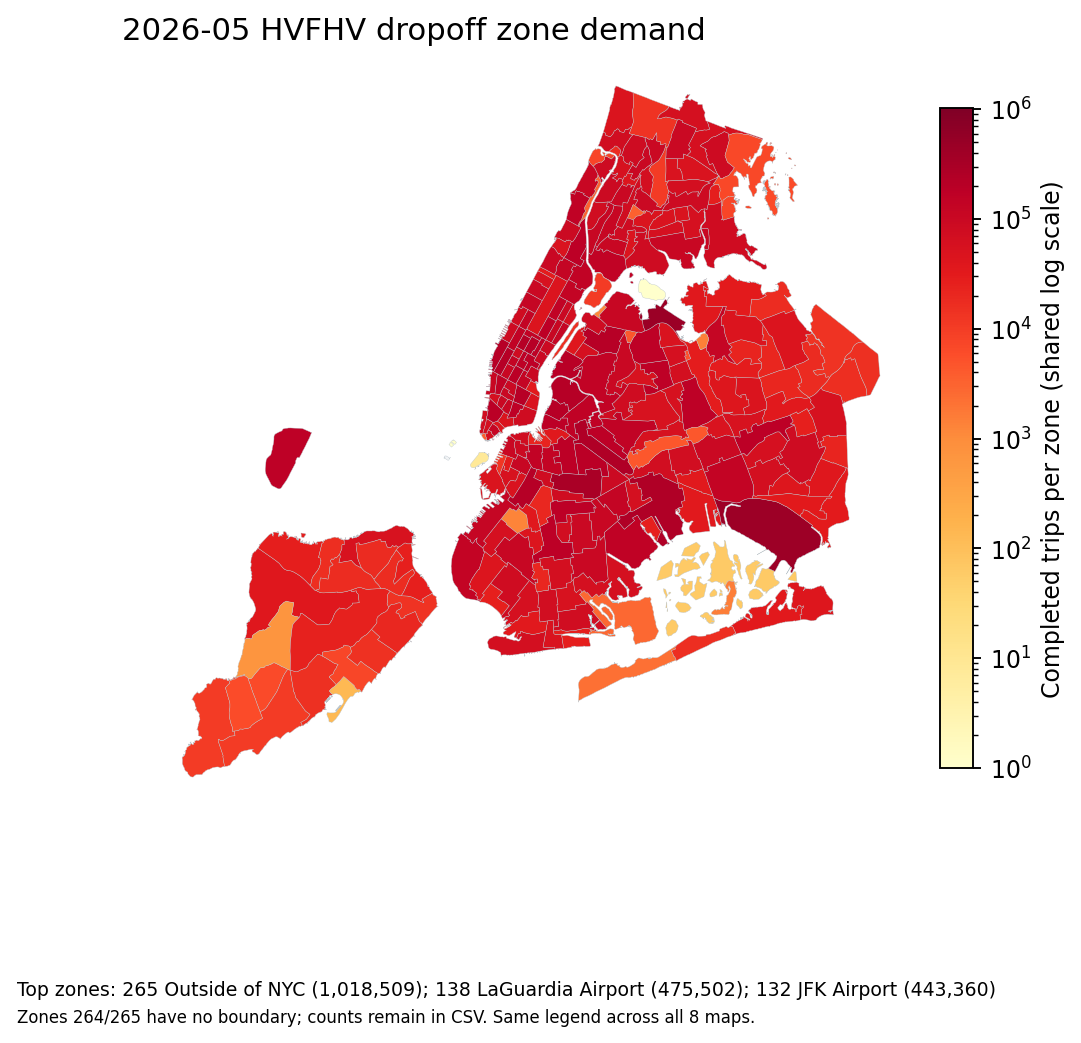
\includegraphics[width=.83\textwidth,height=.72\textheight,keepaspectratio]{04_Results/Task_2/figures/hotspot_2026-05_hvfhv_dropoff.png}
\caption{2026-05 HVFHV dropoff counts by TLC zone. The color shows completed trip records, not people or all requests. Zones 264 and 265 have no polygon; their counts remain in the CSV.}\label{fig:hot05hDO}
\end{figure}

\clearpage\subsection{Directed top-ten OD flows}

\begin{figure}[p]\centering
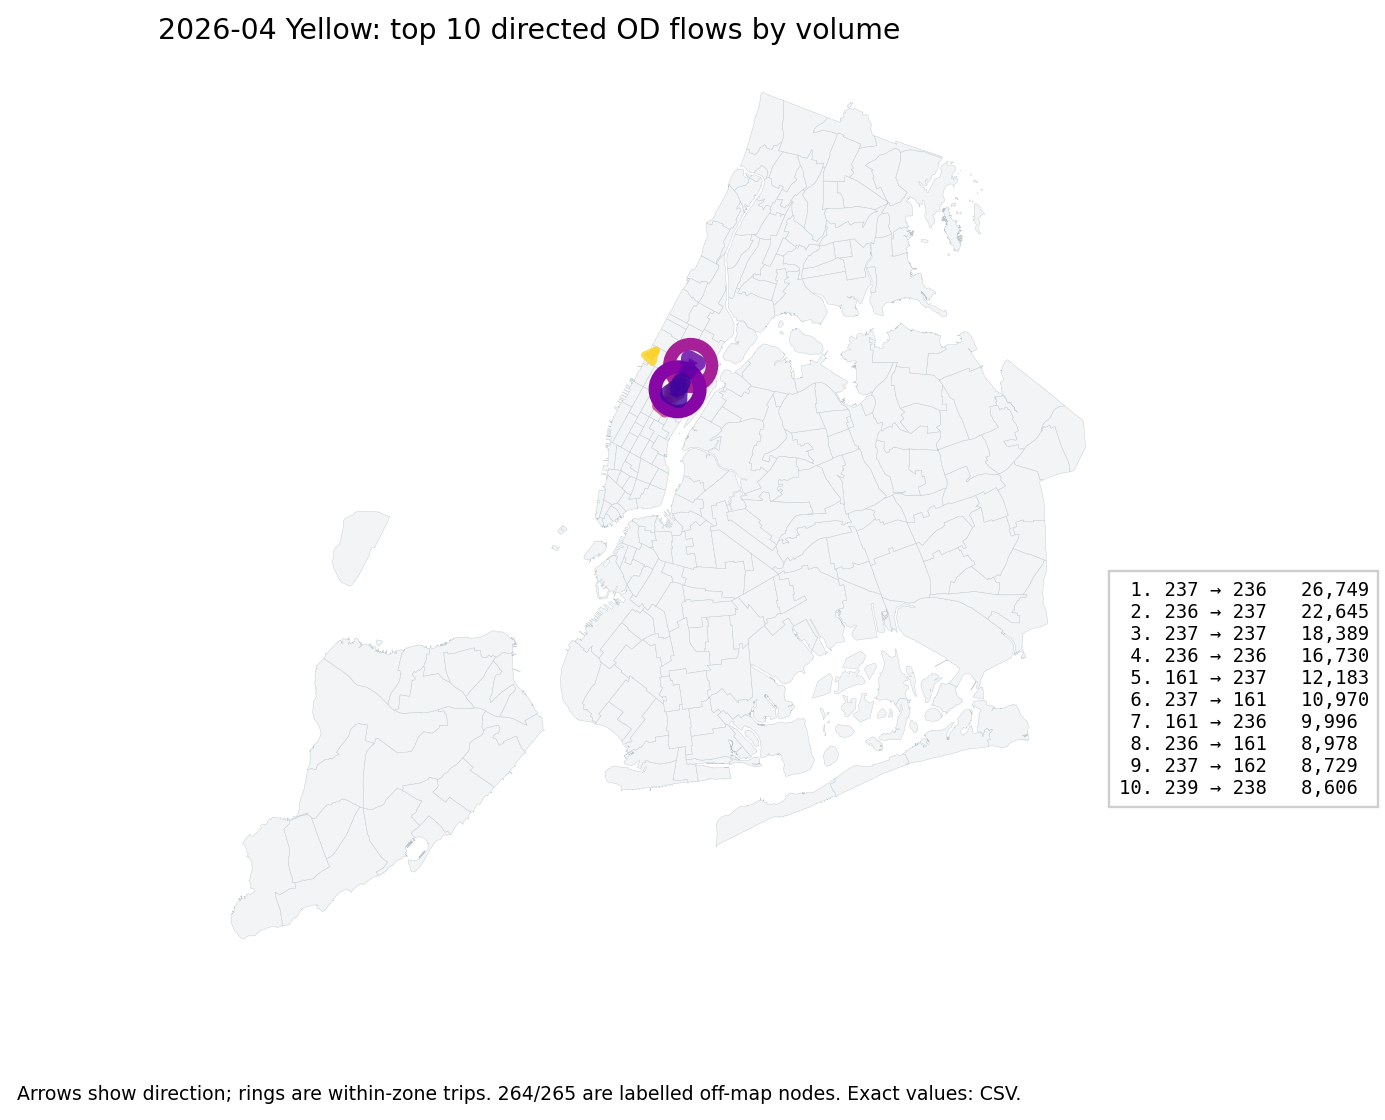
\includegraphics[width=.83\textwidth,height=.72\textheight,keepaspectratio]{04_Results/Task_2/figures/od_volume_2026-04_yellow.png}
\caption{2026-04 Yellow Taxi ten directed OD flows ranked by trip count. Arrows encode OD direction and rings show within-zone trips. Lines join zone centroids, not actual routes.}\label{fig:od04yV}
\end{figure}

\begin{figure}[p]\centering
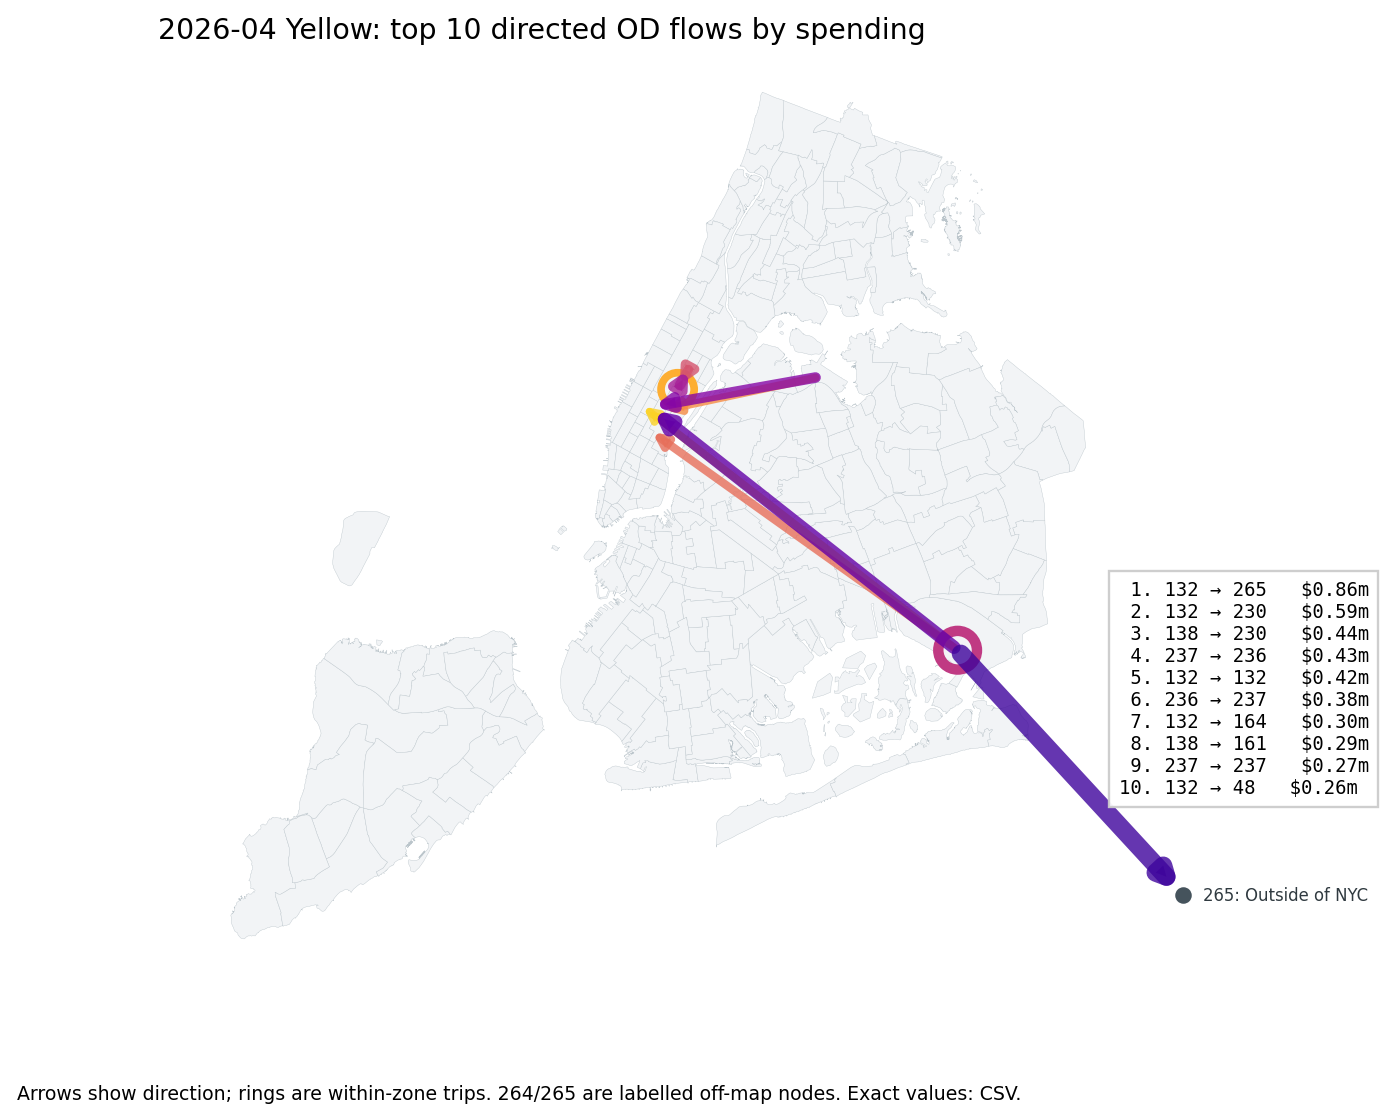
\includegraphics[width=.83\textwidth,height=.72\textheight,keepaspectratio]{04_Results/Task_2/figures/od_spending_2026-04_yellow.png}
\caption{2026-04 Yellow Taxi ten directed OD flows ranked by total valid passenger spending. Arrows encode OD direction and rings show within-zone trips. Lines join zone centroids, not actual routes.}\label{fig:od04yS}
\end{figure}

\begin{figure}[p]\centering
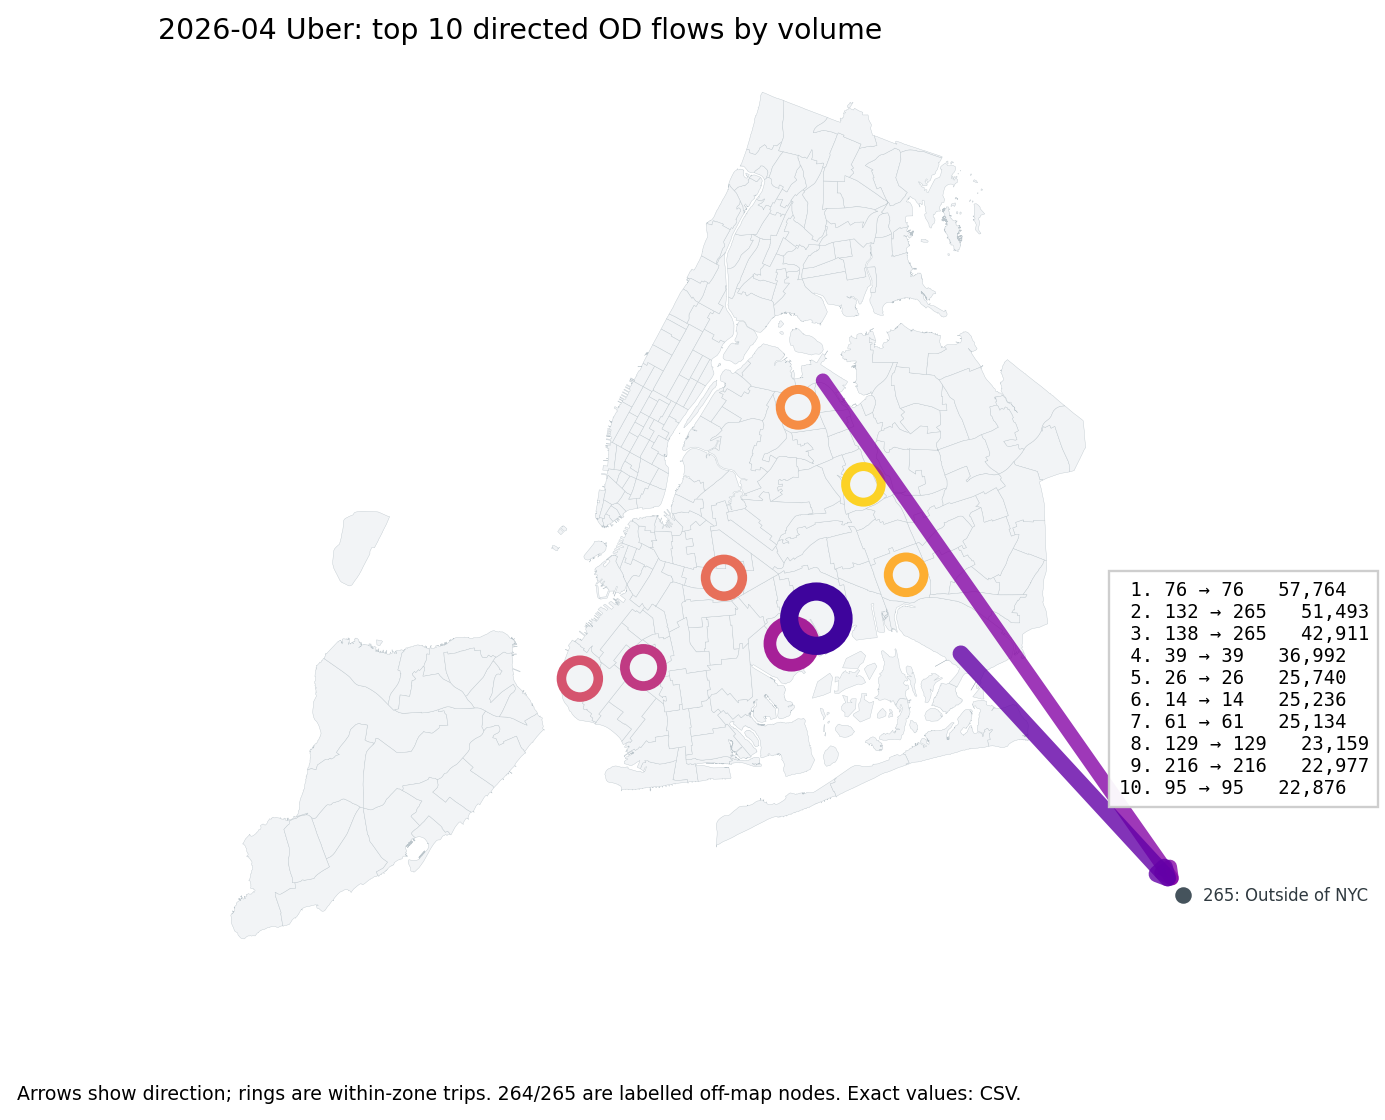
\includegraphics[width=.83\textwidth,height=.72\textheight,keepaspectratio]{04_Results/Task_2/figures/od_volume_2026-04_uber.png}
\caption{2026-04 Uber ten directed OD flows ranked by trip count. Arrows encode OD direction and rings show within-zone trips. Lines join zone centroids, not actual routes.}\label{fig:od04uV}
\end{figure}

\begin{figure}[p]\centering
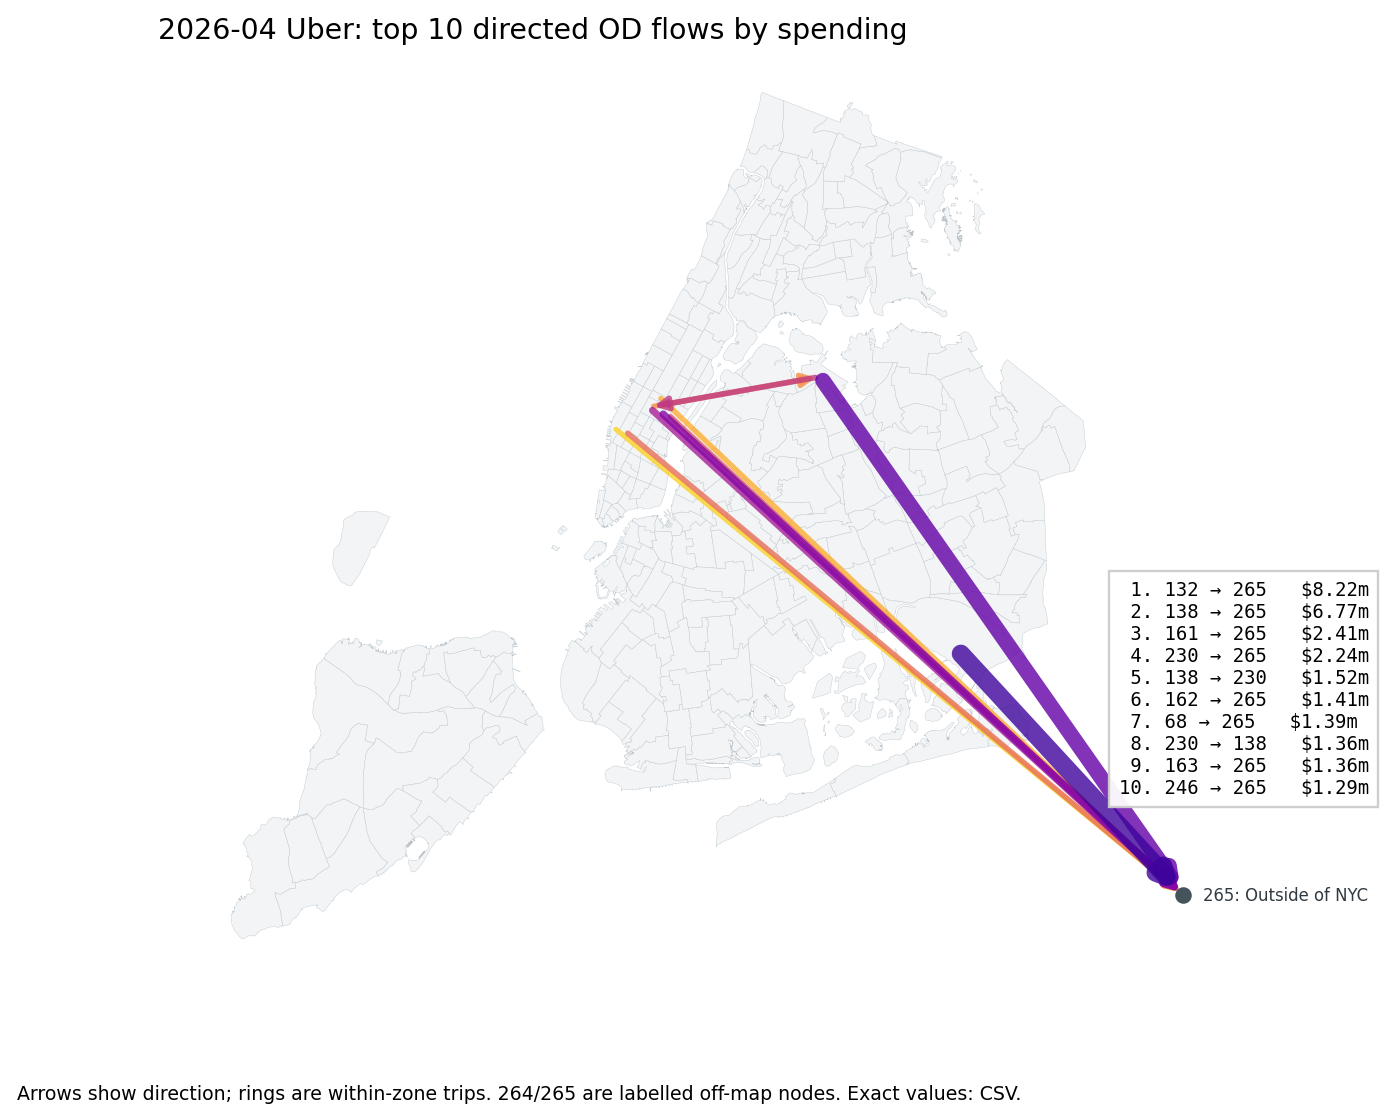
\includegraphics[width=.83\textwidth,height=.72\textheight,keepaspectratio]{04_Results/Task_2/figures/od_spending_2026-04_uber.png}
\caption{2026-04 Uber ten directed OD flows ranked by total valid passenger spending. Arrows encode OD direction and rings show within-zone trips. Lines join zone centroids, not actual routes.}\label{fig:od04uS}
\end{figure}

\begin{figure}[p]\centering
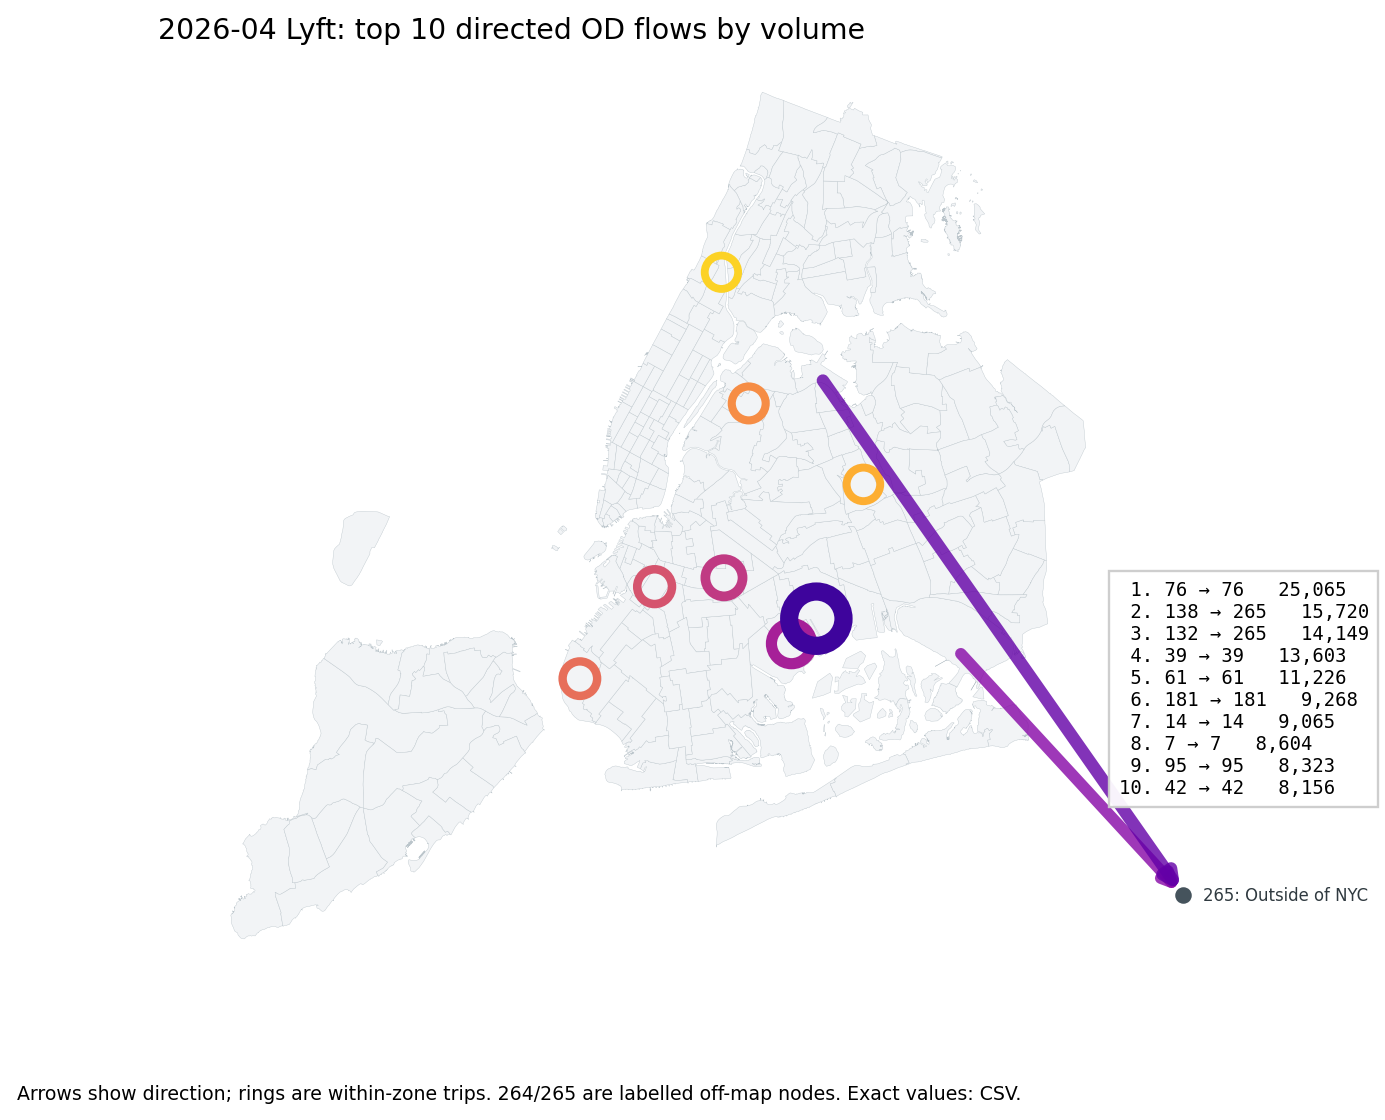
\includegraphics[width=.83\textwidth,height=.72\textheight,keepaspectratio]{04_Results/Task_2/figures/od_volume_2026-04_lyft.png}
\caption{2026-04 Lyft ten directed OD flows ranked by trip count. Arrows encode OD direction and rings show within-zone trips. Lines join zone centroids, not actual routes.}\label{fig:od04lV}
\end{figure}

\begin{figure}[p]\centering
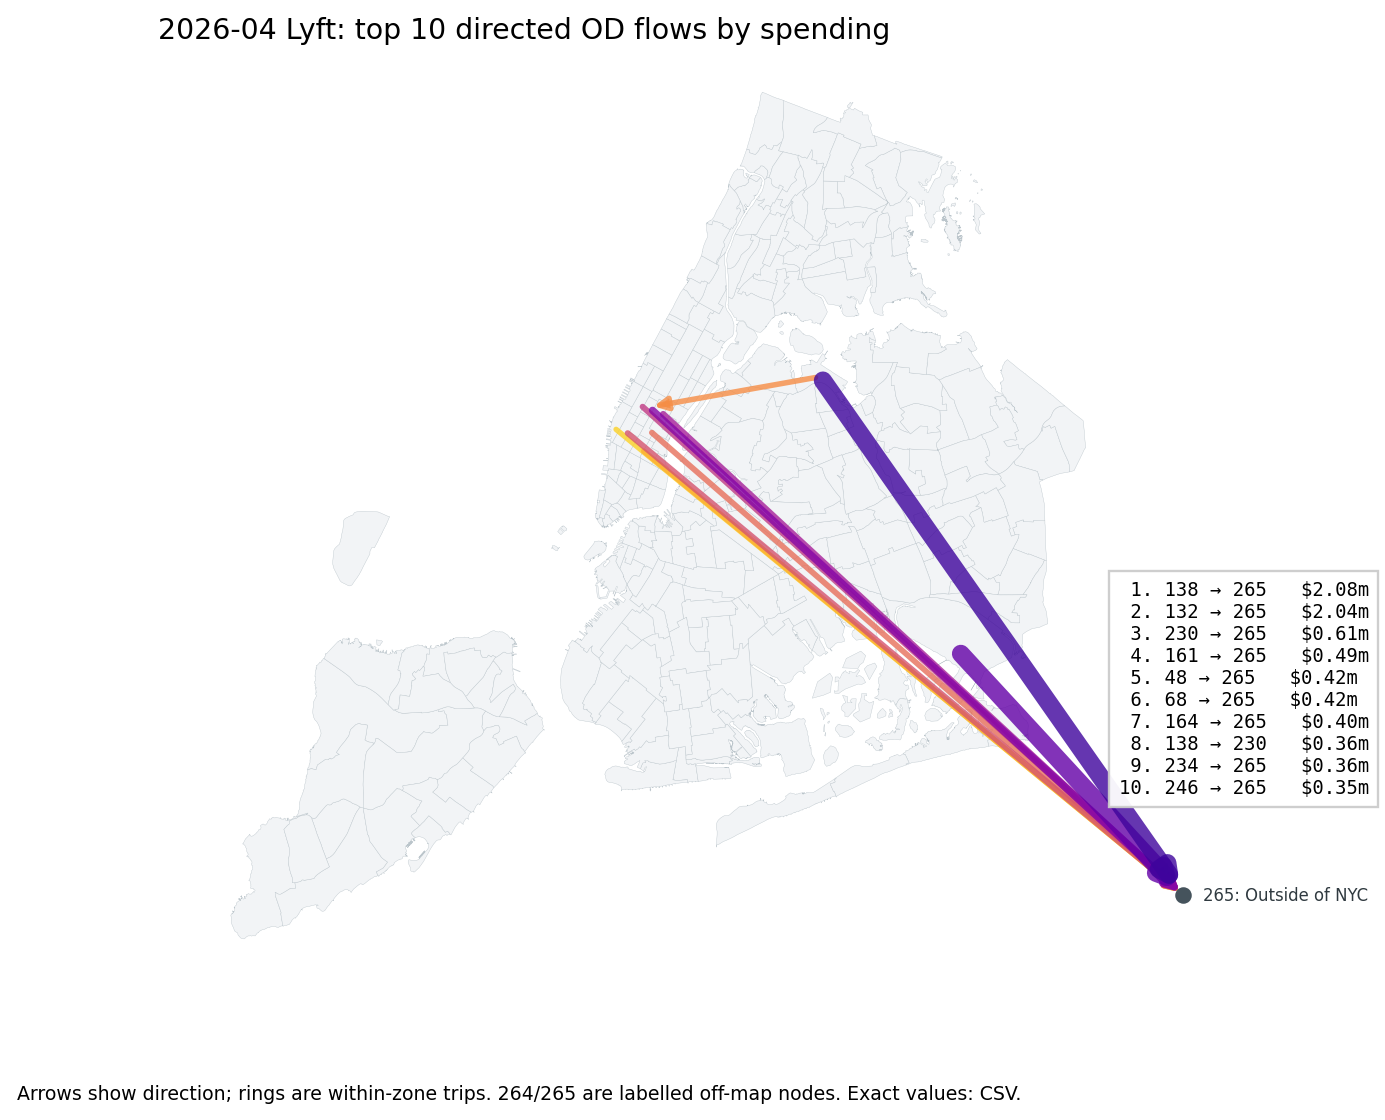
\includegraphics[width=.83\textwidth,height=.72\textheight,keepaspectratio]{04_Results/Task_2/figures/od_spending_2026-04_lyft.png}
\caption{2026-04 Lyft ten directed OD flows ranked by total valid passenger spending. Arrows encode OD direction and rings show within-zone trips. Lines join zone centroids, not actual routes.}\label{fig:od04lS}
\end{figure}

\begin{figure}[p]\centering
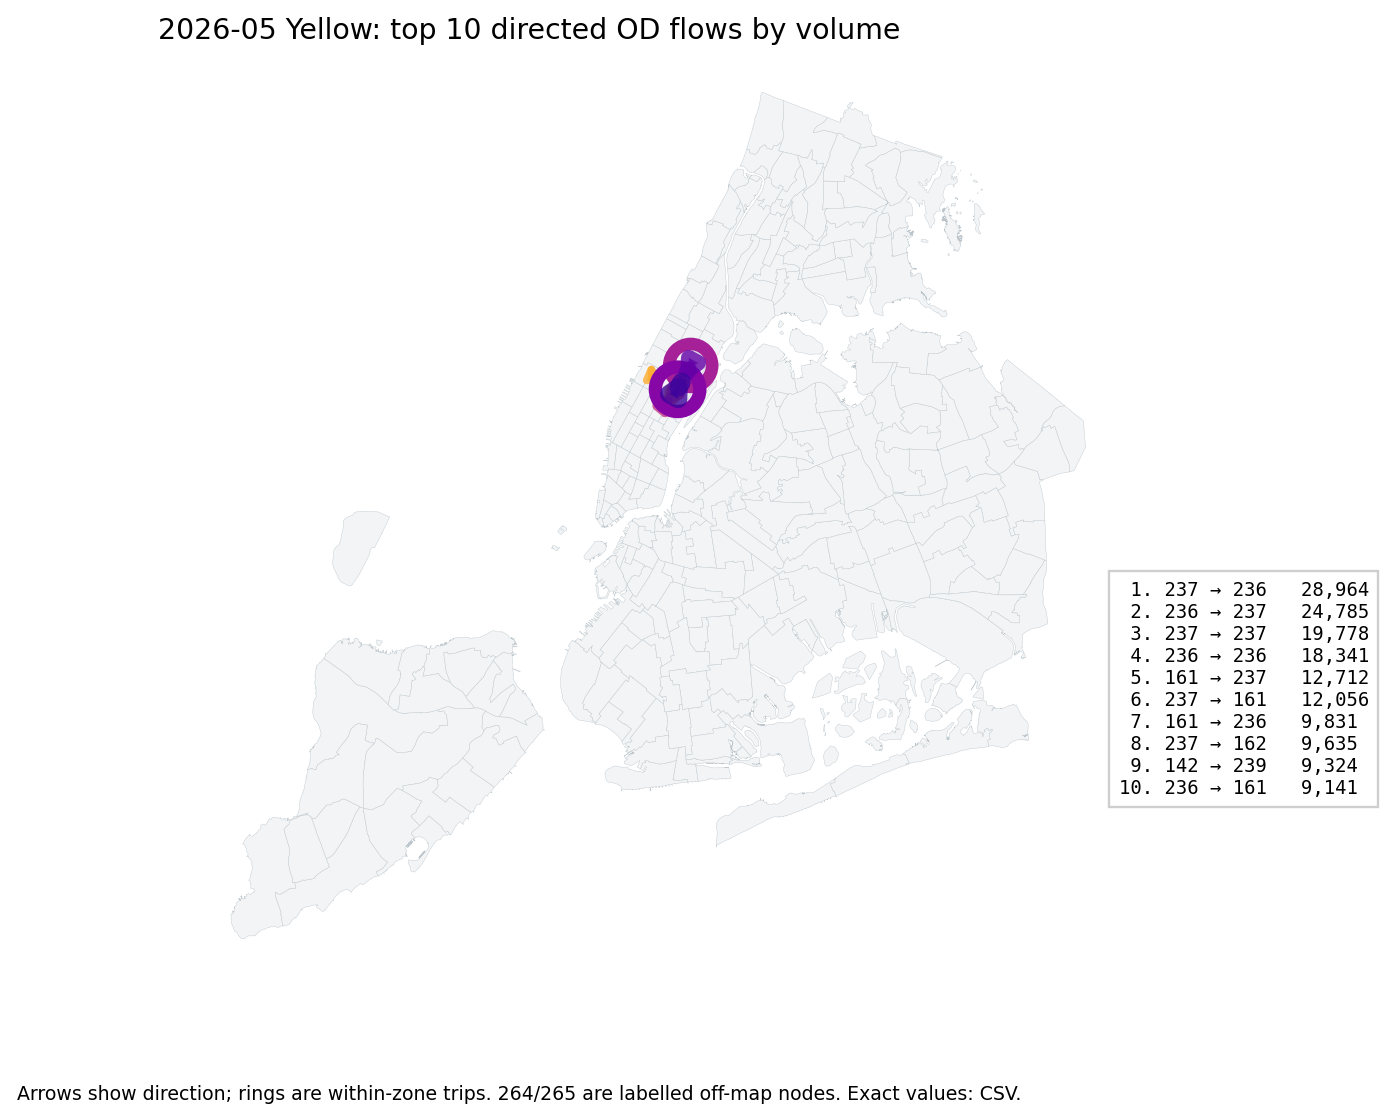
\includegraphics[width=.83\textwidth,height=.72\textheight,keepaspectratio]{04_Results/Task_2/figures/od_volume_2026-05_yellow.png}
\caption{2026-05 Yellow Taxi ten directed OD flows ranked by trip count. Arrows encode OD direction and rings show within-zone trips. Lines join zone centroids, not actual routes.}\label{fig:od05yV}
\end{figure}

\begin{figure}[p]\centering
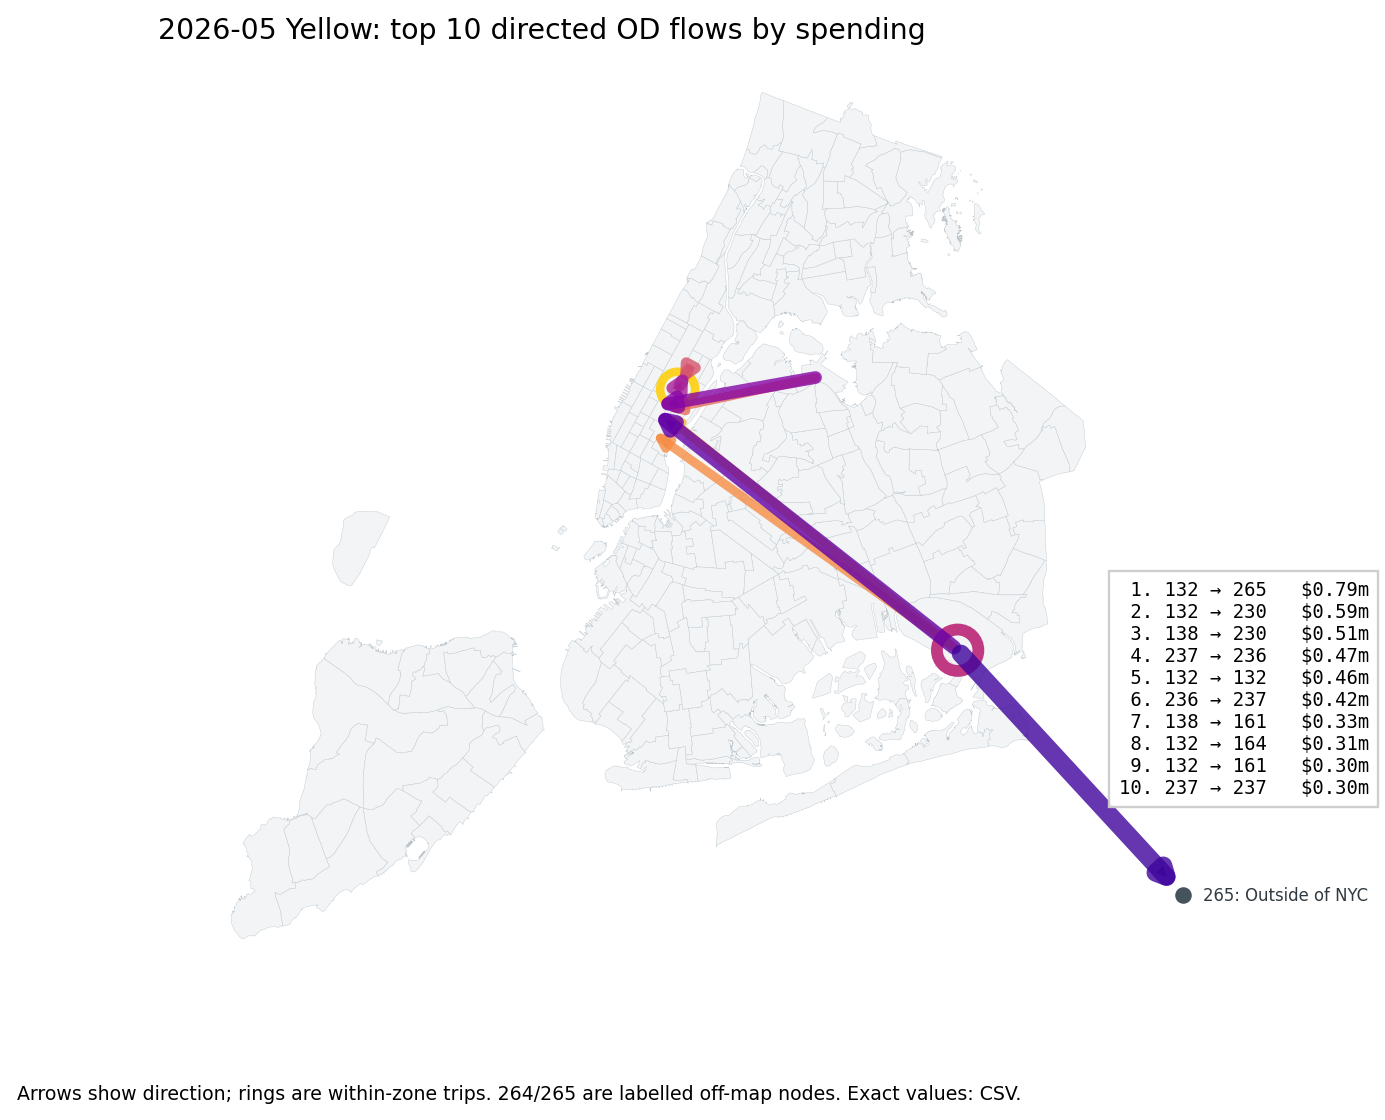
\includegraphics[width=.83\textwidth,height=.72\textheight,keepaspectratio]{04_Results/Task_2/figures/od_spending_2026-05_yellow.png}
\caption{2026-05 Yellow Taxi ten directed OD flows ranked by total valid passenger spending. Arrows encode OD direction and rings show within-zone trips. Lines join zone centroids, not actual routes.}\label{fig:od05yS}
\end{figure}

\begin{figure}[p]\centering
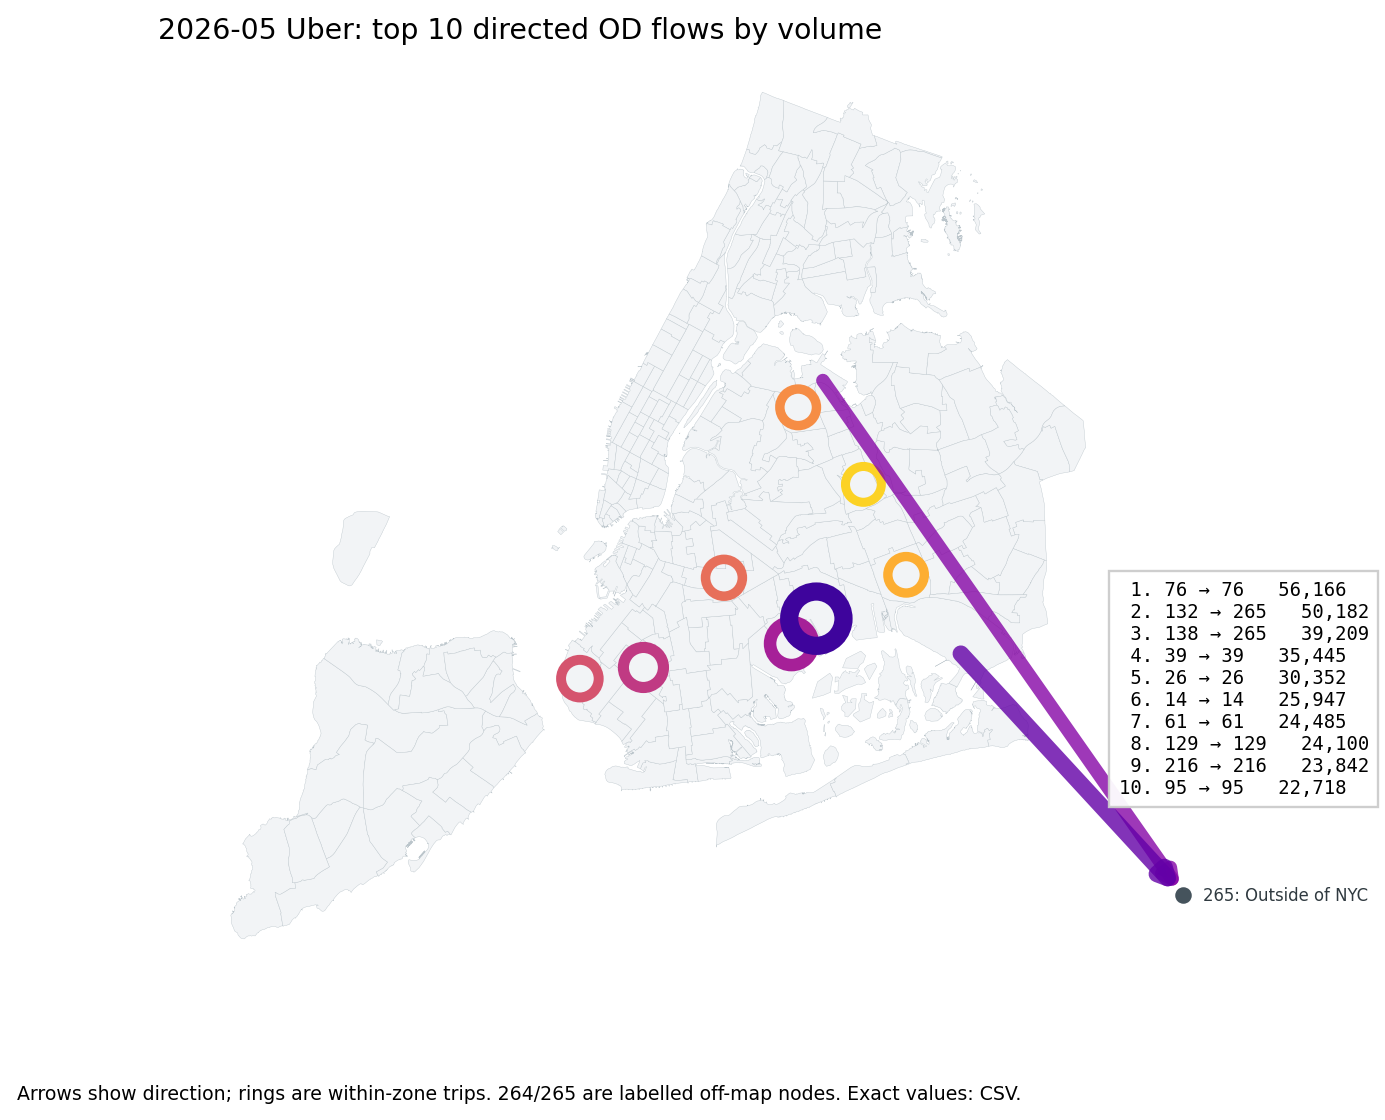
\includegraphics[width=.83\textwidth,height=.72\textheight,keepaspectratio]{04_Results/Task_2/figures/od_volume_2026-05_uber.png}
\caption{2026-05 Uber ten directed OD flows ranked by trip count. Arrows encode OD direction and rings show within-zone trips. Lines join zone centroids, not actual routes.}\label{fig:od05uV}
\end{figure}

\begin{figure}[p]\centering
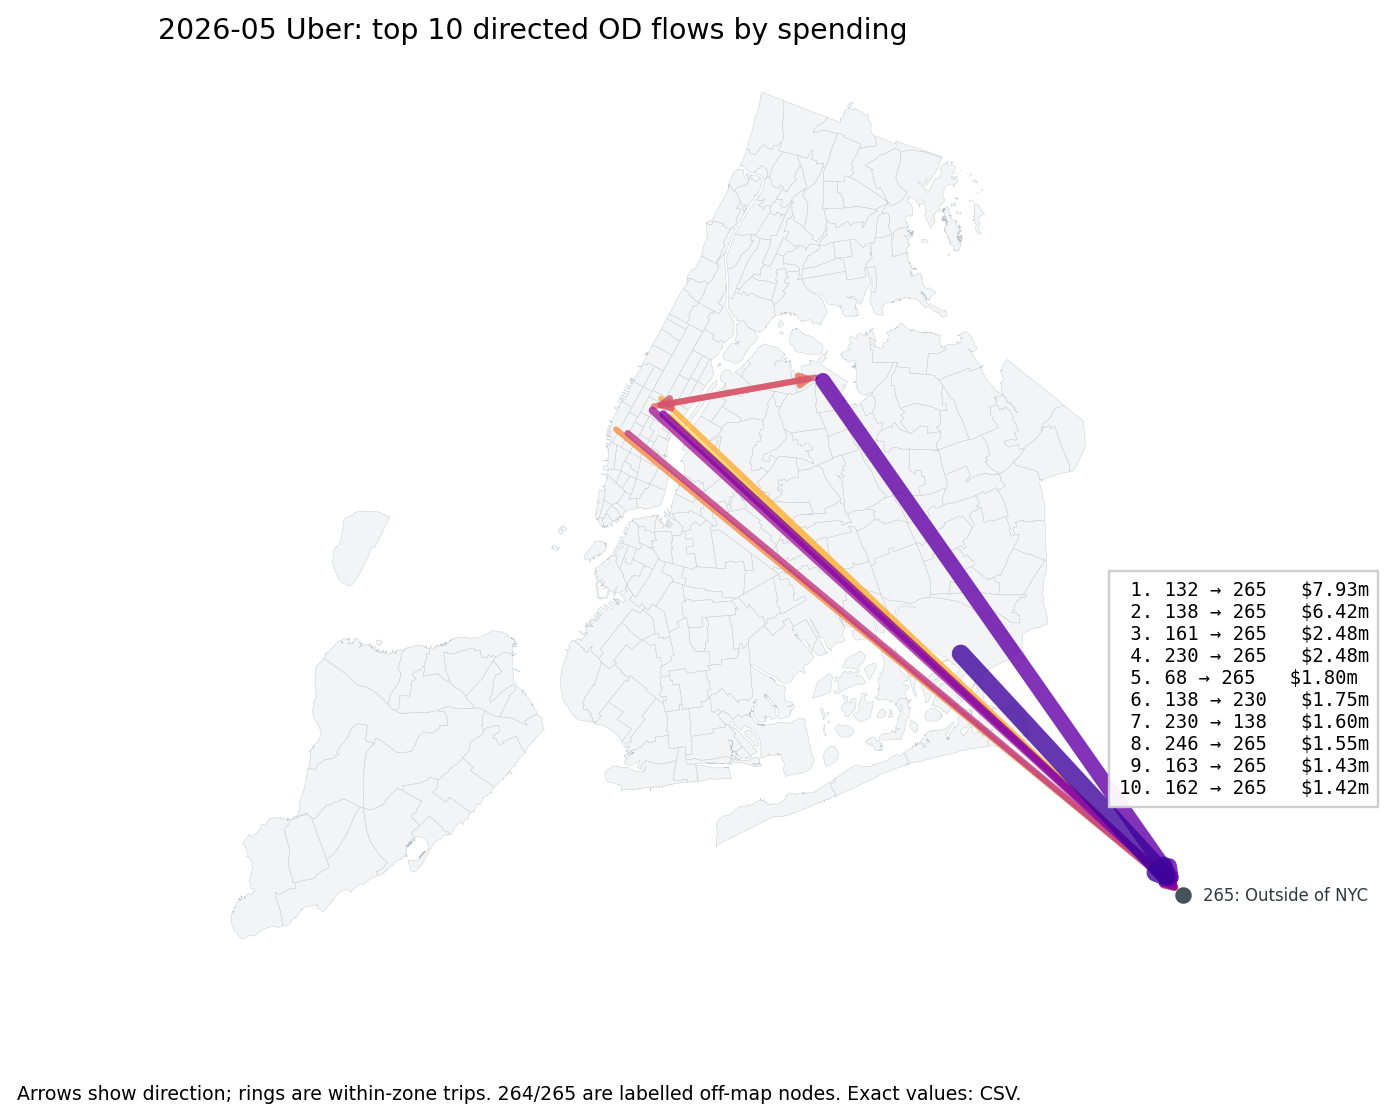
\includegraphics[width=.83\textwidth,height=.72\textheight,keepaspectratio]{04_Results/Task_2/figures/od_spending_2026-05_uber.png}
\caption{2026-05 Uber ten directed OD flows ranked by total valid passenger spending. Arrows encode OD direction and rings show within-zone trips. Lines join zone centroids, not actual routes.}\label{fig:od05uS}
\end{figure}

\begin{figure}[p]\centering
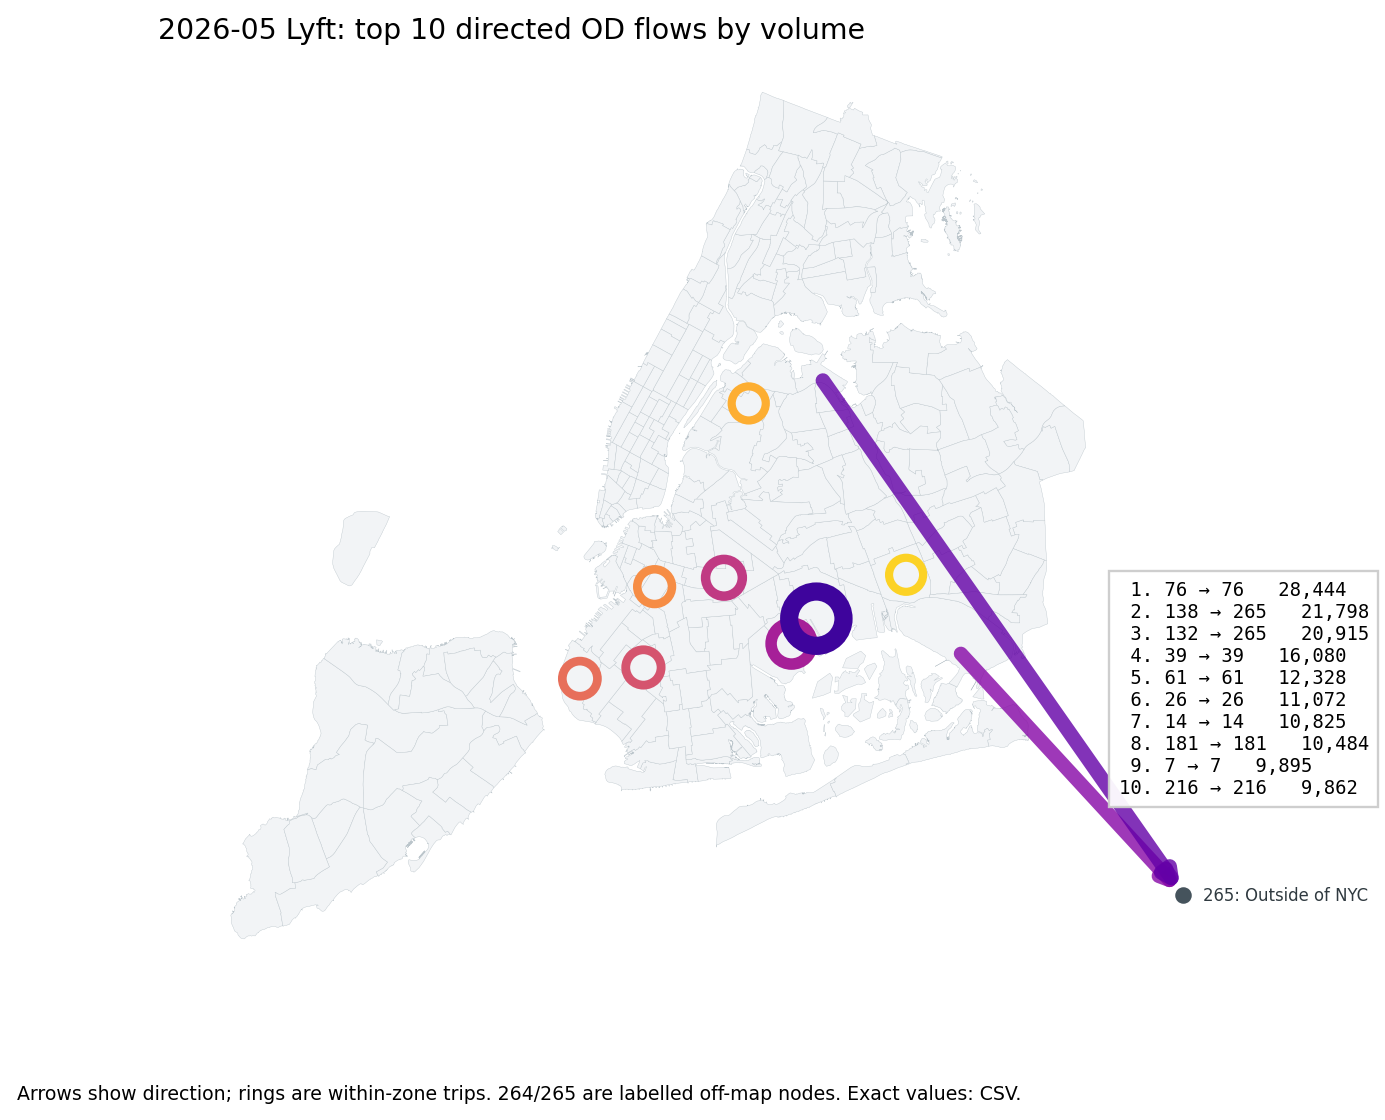
\includegraphics[width=.83\textwidth,height=.72\textheight,keepaspectratio]{04_Results/Task_2/figures/od_volume_2026-05_lyft.png}
\caption{2026-05 Lyft ten directed OD flows ranked by trip count. Arrows encode OD direction and rings show within-zone trips. Lines join zone centroids, not actual routes.}\label{fig:od05lV}
\end{figure}

\begin{figure}[p]\centering
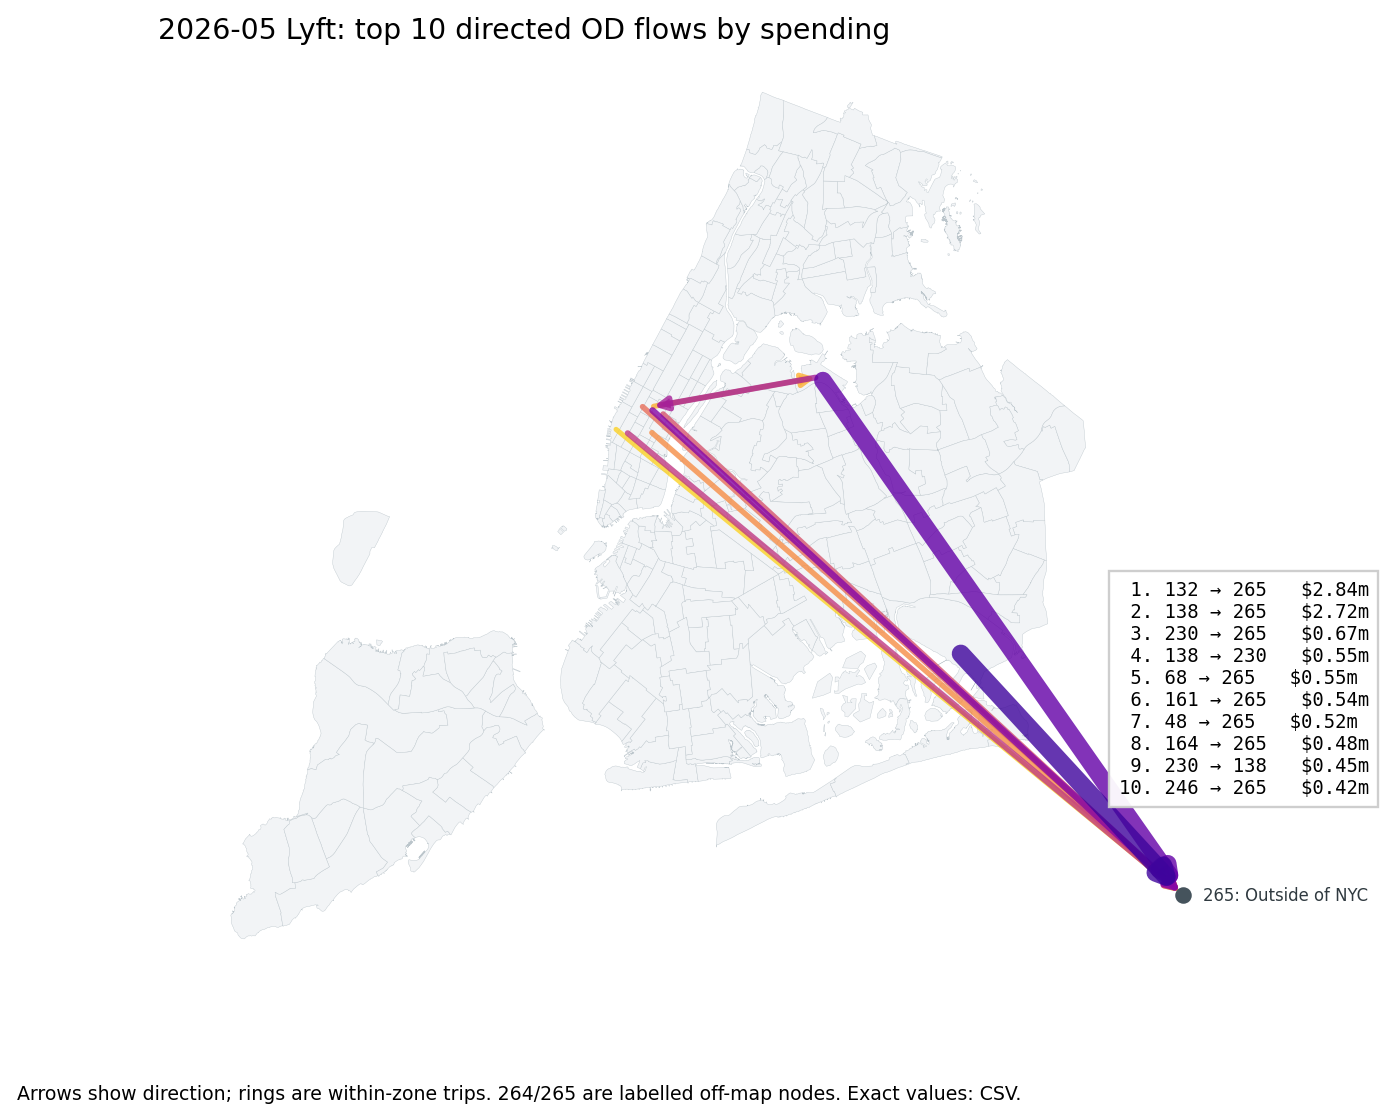
\includegraphics[width=.83\textwidth,height=.72\textheight,keepaspectratio]{04_Results/Task_2/figures/od_spending_2026-05_lyft.png}
\caption{2026-05 Lyft ten directed OD flows ranked by total valid passenger spending. Arrows encode OD direction and rings show within-zone trips. Lines join zone centroids, not actual routes.}\label{fig:od05lS}
\end{figure}

\clearpage\subsection{Reported sharing by pickup zone}

\begin{figure}[p]\centering
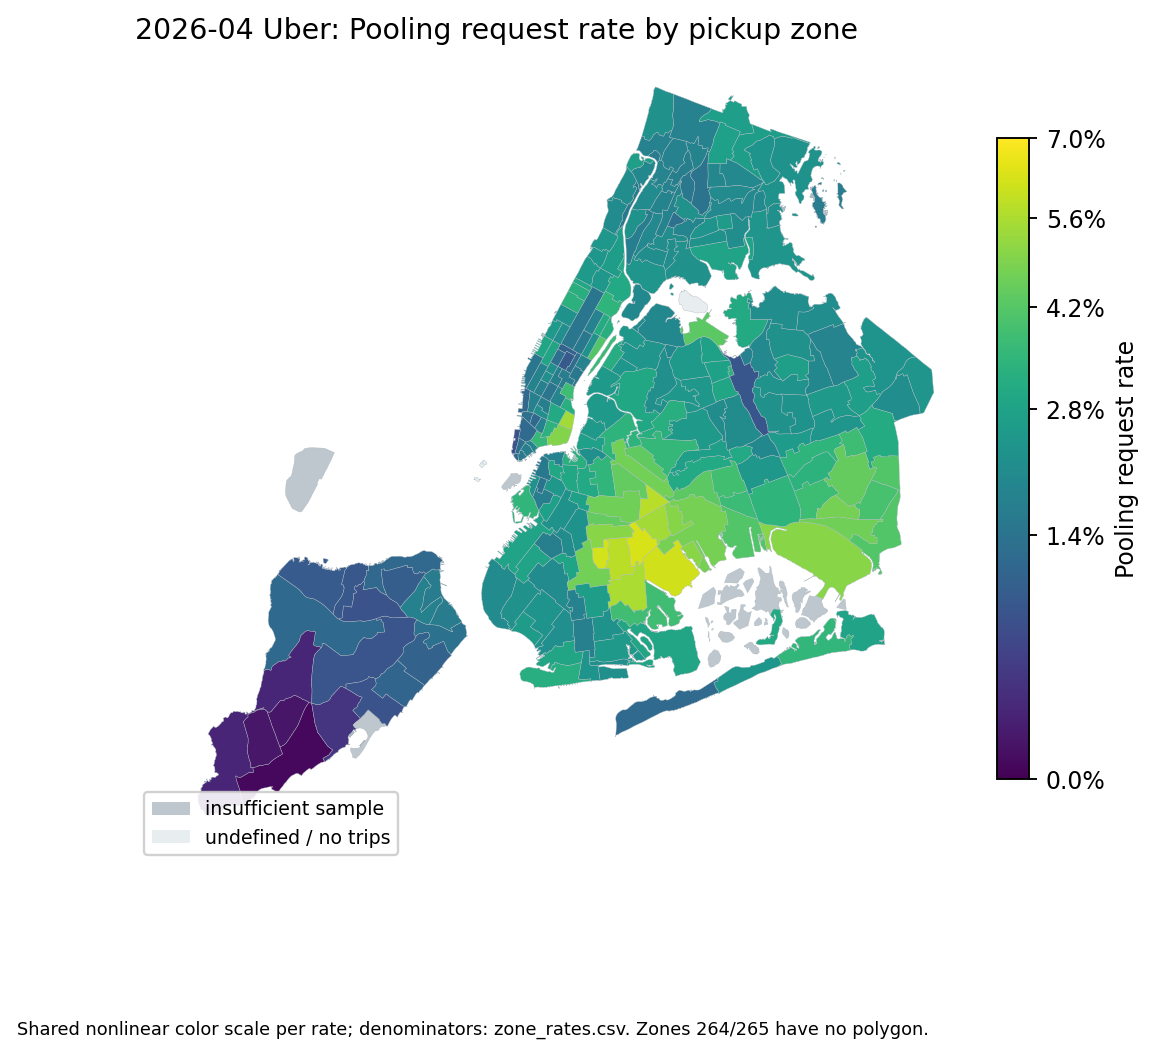
\includegraphics[width=.83\textwidth,height=.72\textheight,keepaspectratio]{04_Results/Task_3/figures/pooling_request_rate_2026-04_uber.png}
\caption{2026-04 Uber pooling request rate by pickup zone, denominator: valid-status trips. Gray zones have fewer than 100 valid-status trips; pale zones have an undefined rate. A gray zone is not a measured zero rate.}\label{fig:share04uQ}
\end{figure}

\begin{figure}[p]\centering
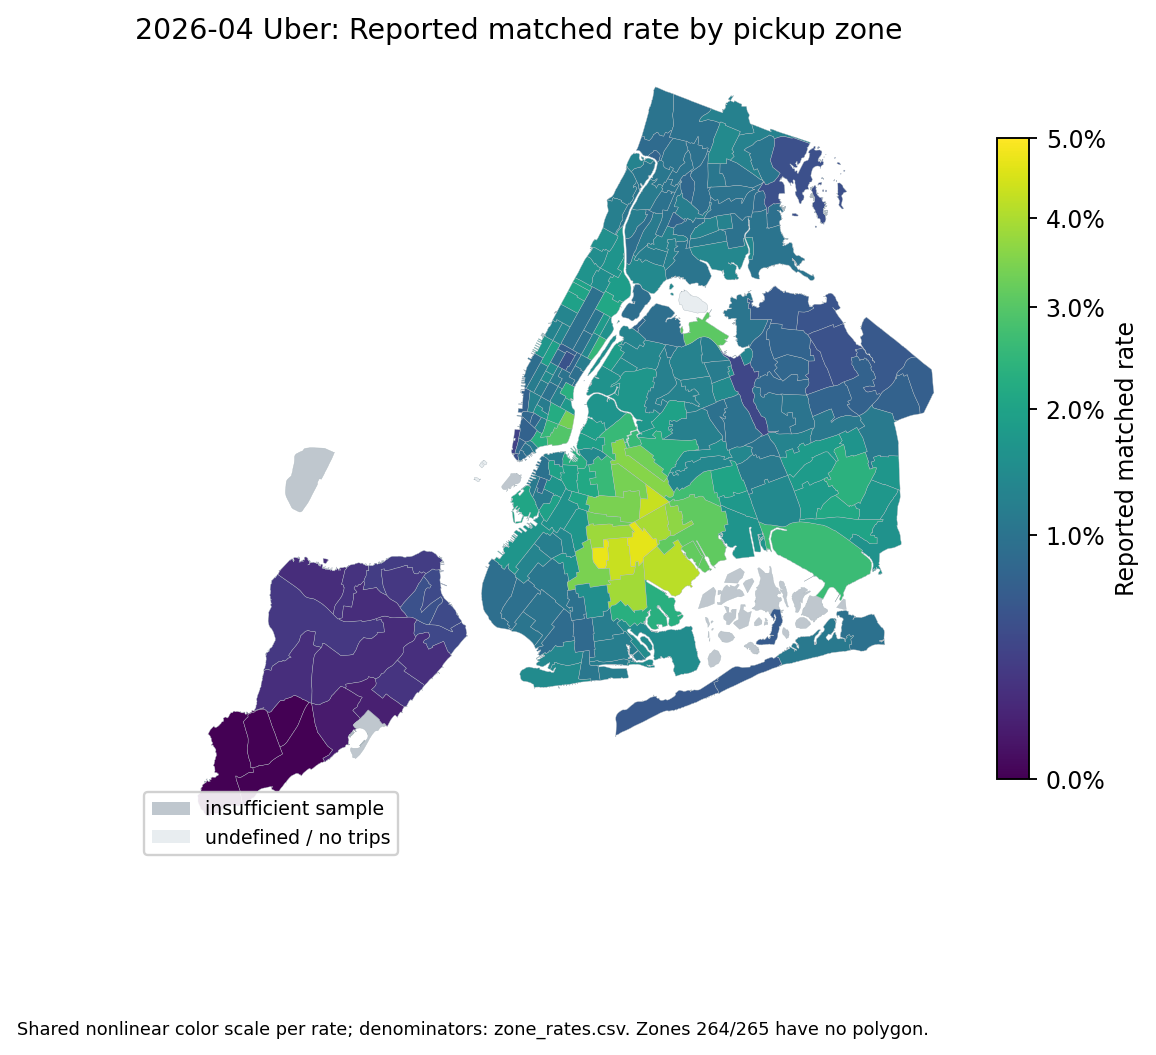
\includegraphics[width=.83\textwidth,height=.72\textheight,keepaspectratio]{04_Results/Task_3/figures/reported_matched_rate_2026-04_uber.png}
\caption{2026-04 Uber reported matched rate by pickup zone, denominator: valid-status trips. Gray zones have fewer than 100 valid-status trips; pale zones have an undefined rate. A gray zone is not a measured zero rate.}\label{fig:share04uM}
\end{figure}

\begin{figure}[p]\centering
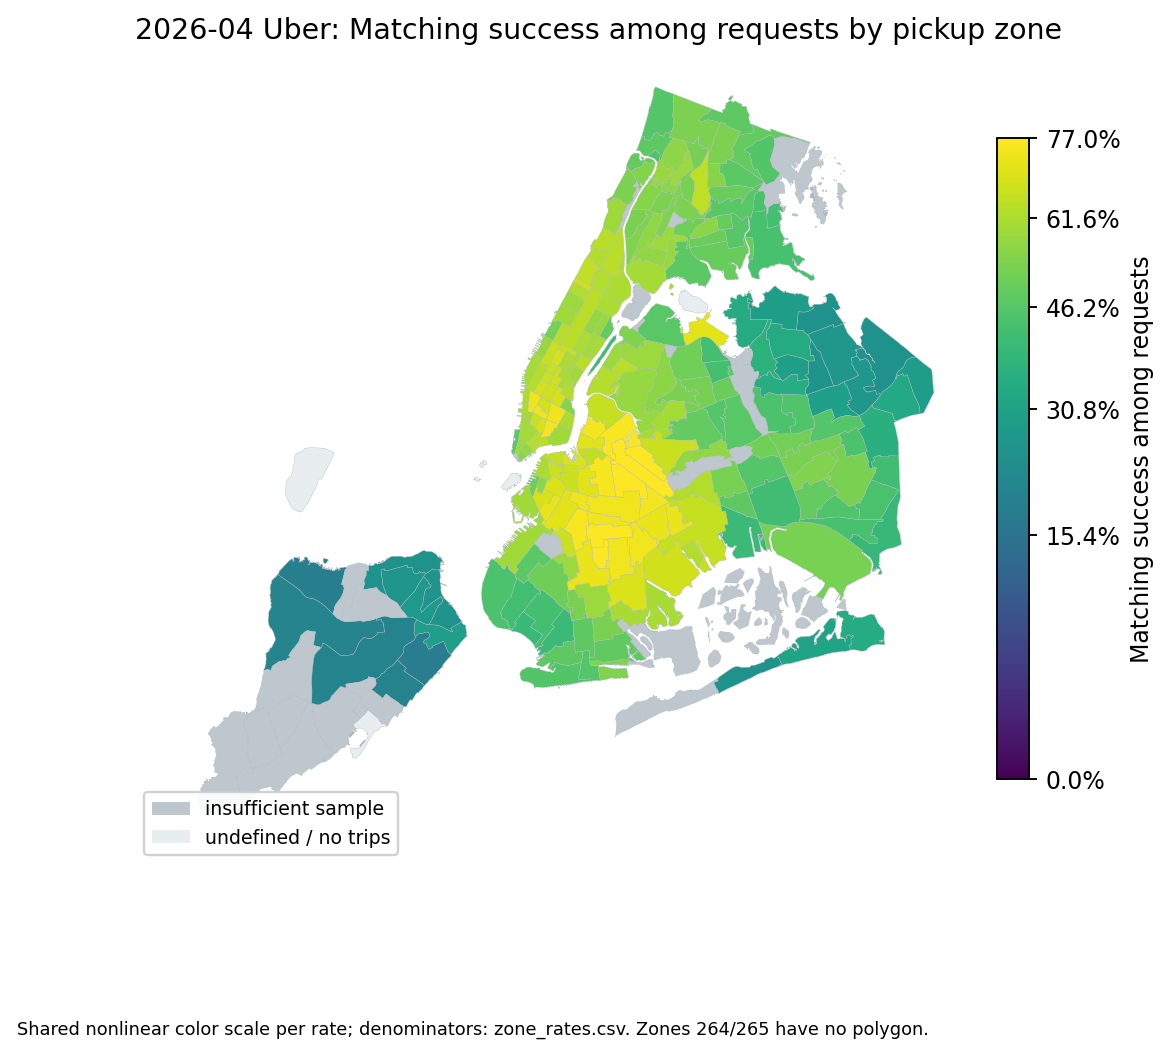
\includegraphics[width=.83\textwidth,height=.72\textheight,keepaspectratio]{04_Results/Task_3/figures/matching_success_2026-04_uber.png}
\caption{2026-04 Uber matching success among pooling requests by pickup zone. Only 232 zones meet the 100-request reporting threshold; gray zones have insufficient requests and pale zones have no defined rate. Colors should be read only for reportable zones.}\label{fig:share04uS}
\end{figure}

\begin{figure}[p]\centering
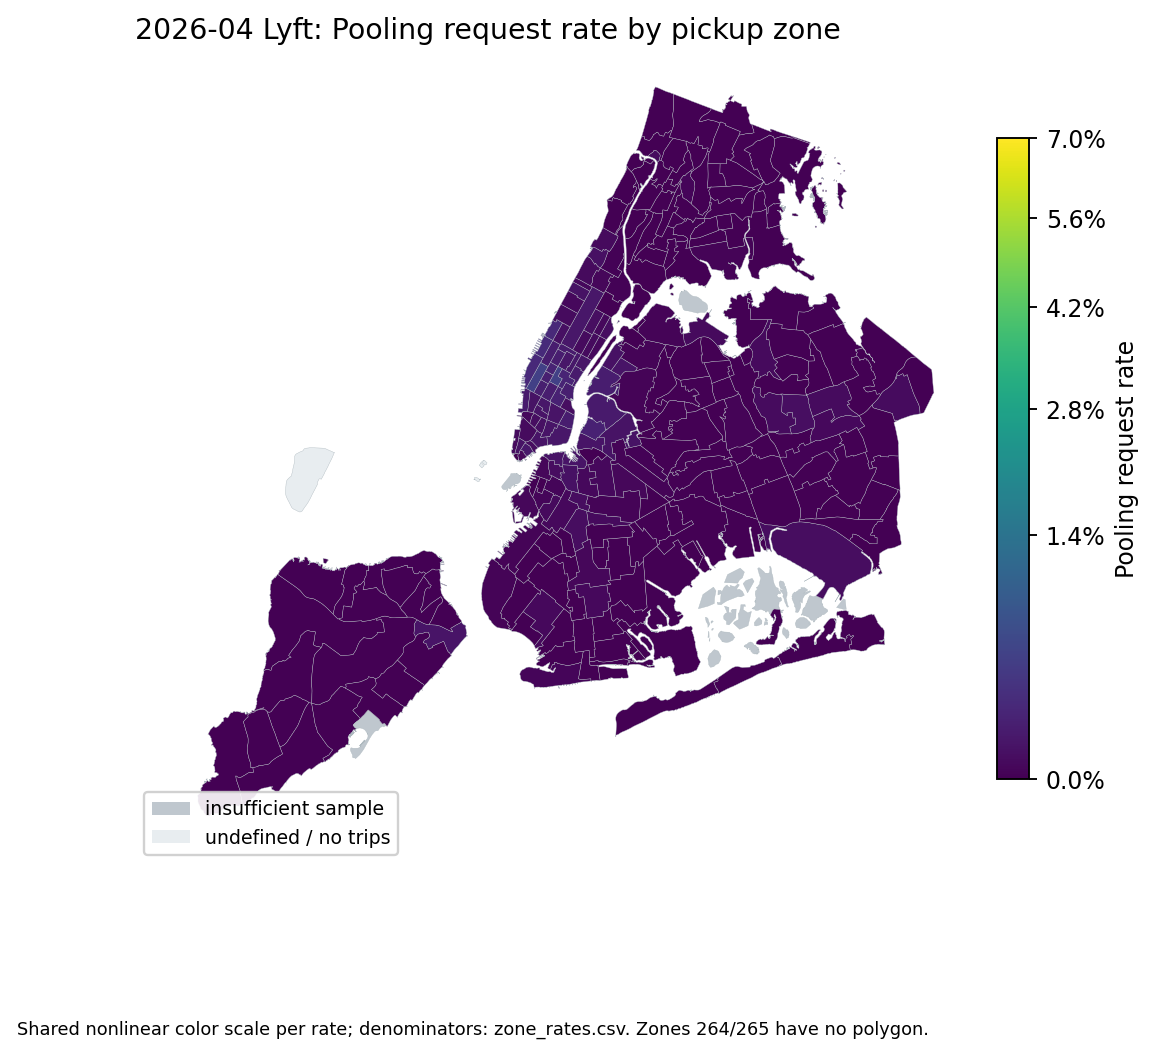
\includegraphics[width=.83\textwidth,height=.72\textheight,keepaspectratio]{04_Results/Task_3/figures/pooling_request_rate_2026-04_lyft.png}
\caption{2026-04 Lyft pooling request rate by pickup zone, denominator: valid-status trips. Gray zones have fewer than 100 valid-status trips; pale zones have an undefined rate. A gray zone is not a measured zero rate.}\label{fig:share04lQ}
\end{figure}

\begin{figure}[p]\centering
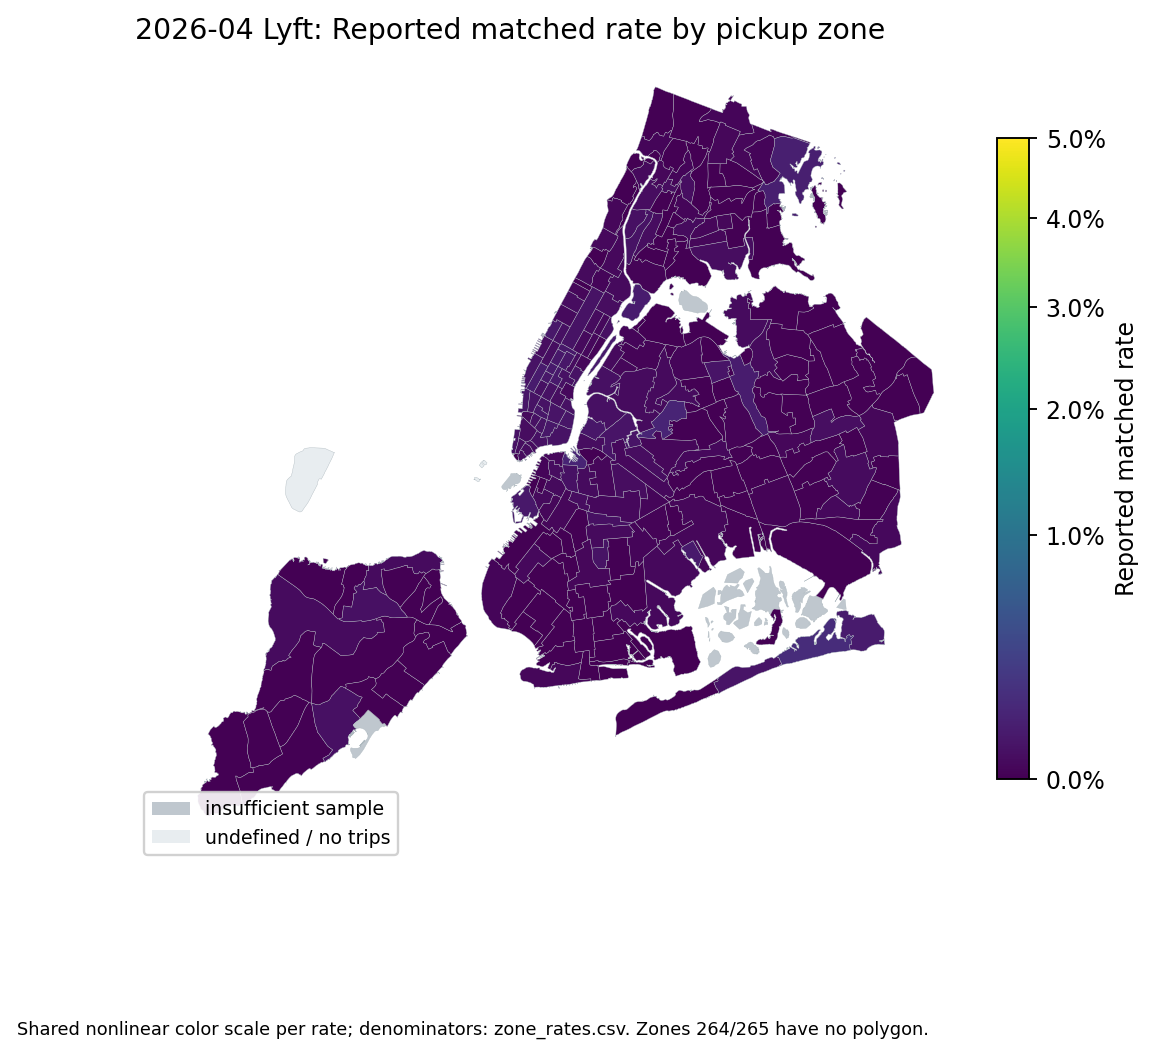
\includegraphics[width=.83\textwidth,height=.72\textheight,keepaspectratio]{04_Results/Task_3/figures/reported_matched_rate_2026-04_lyft.png}
\caption{2026-04 Lyft reported matched rate by pickup zone, denominator: valid-status trips. Gray zones have fewer than 100 valid-status trips; pale zones have an undefined rate. A gray zone is not a measured zero rate.}\label{fig:share04lM}
\end{figure}

\begin{figure}[p]\centering
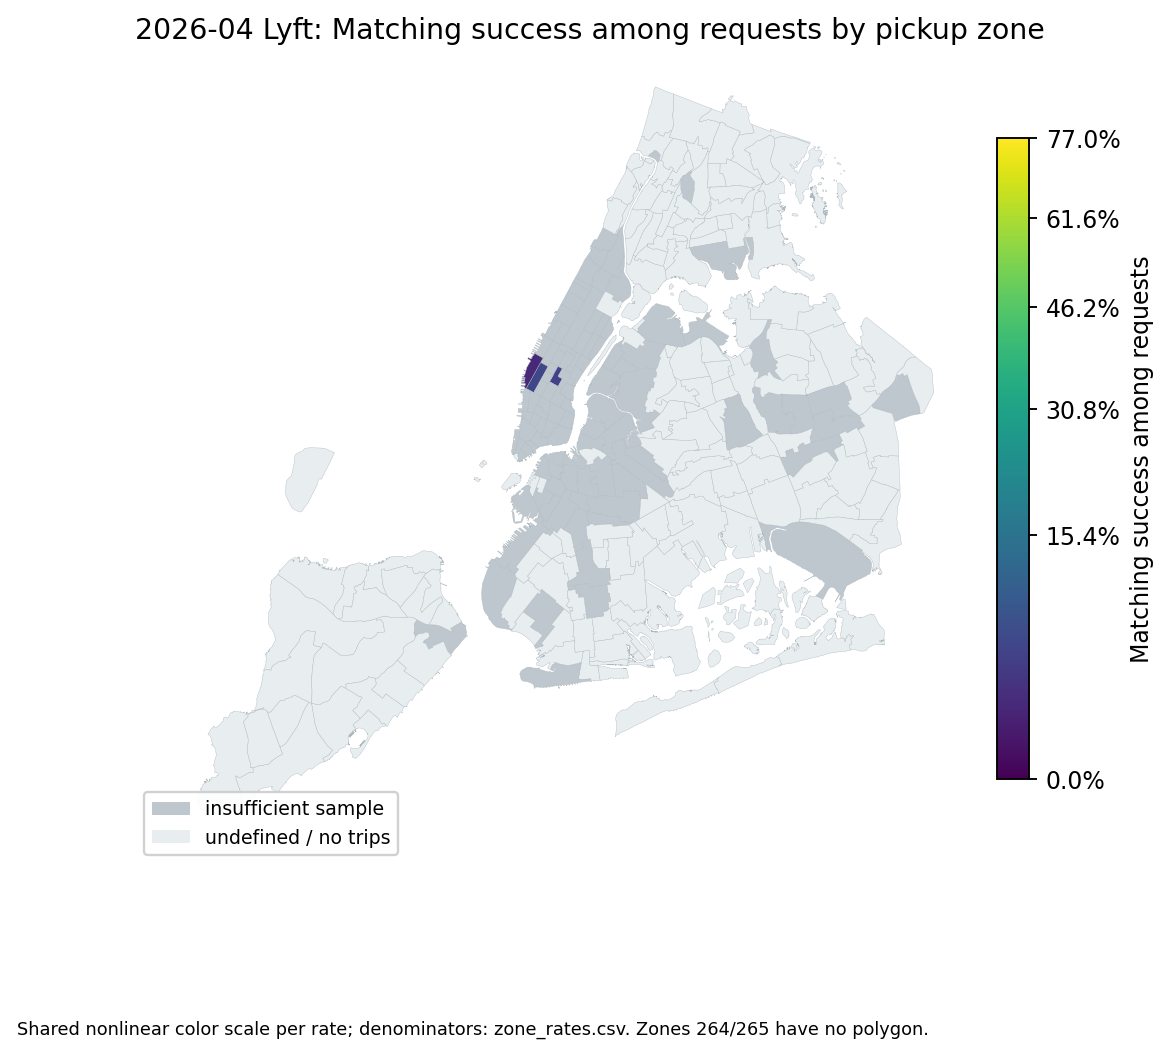
\includegraphics[width=.83\textwidth,height=.72\textheight,keepaspectratio]{04_Results/Task_3/figures/matching_success_2026-04_lyft.png}
\caption{2026-04 Lyft matching success among pooling requests by pickup zone. Only 3 zones meet the 100-request reporting threshold; gray zones have insufficient requests and pale zones have no defined rate. Colors should be read only for reportable zones.}\label{fig:share04lS}
\end{figure}

\begin{figure}[p]\centering
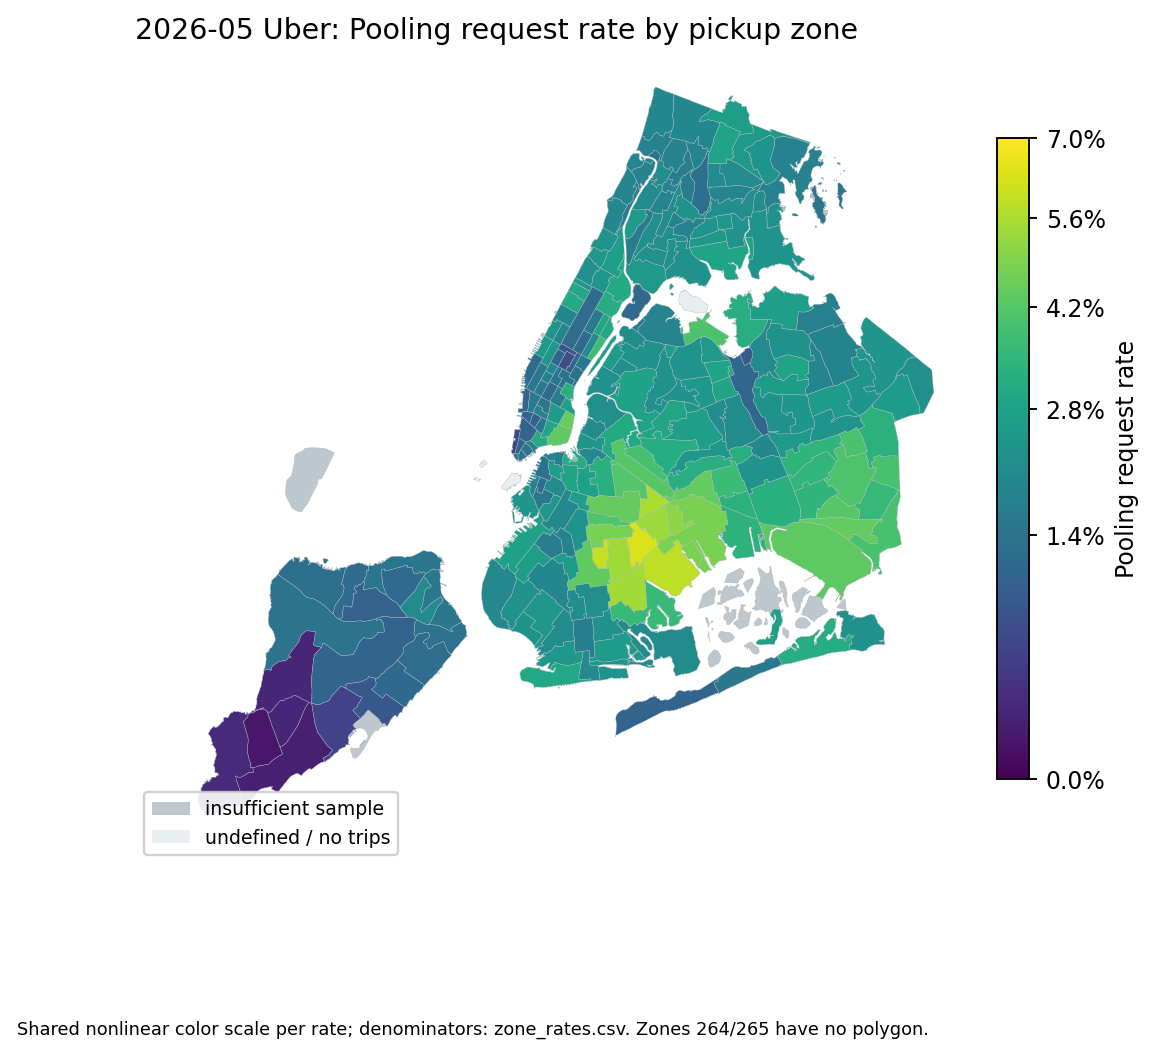
\includegraphics[width=.83\textwidth,height=.72\textheight,keepaspectratio]{04_Results/Task_3/figures/pooling_request_rate_2026-05_uber.png}
\caption{2026-05 Uber pooling request rate by pickup zone, denominator: valid-status trips. Gray zones have fewer than 100 valid-status trips; pale zones have an undefined rate. A gray zone is not a measured zero rate.}\label{fig:share05uQ}
\end{figure}

\begin{figure}[p]\centering
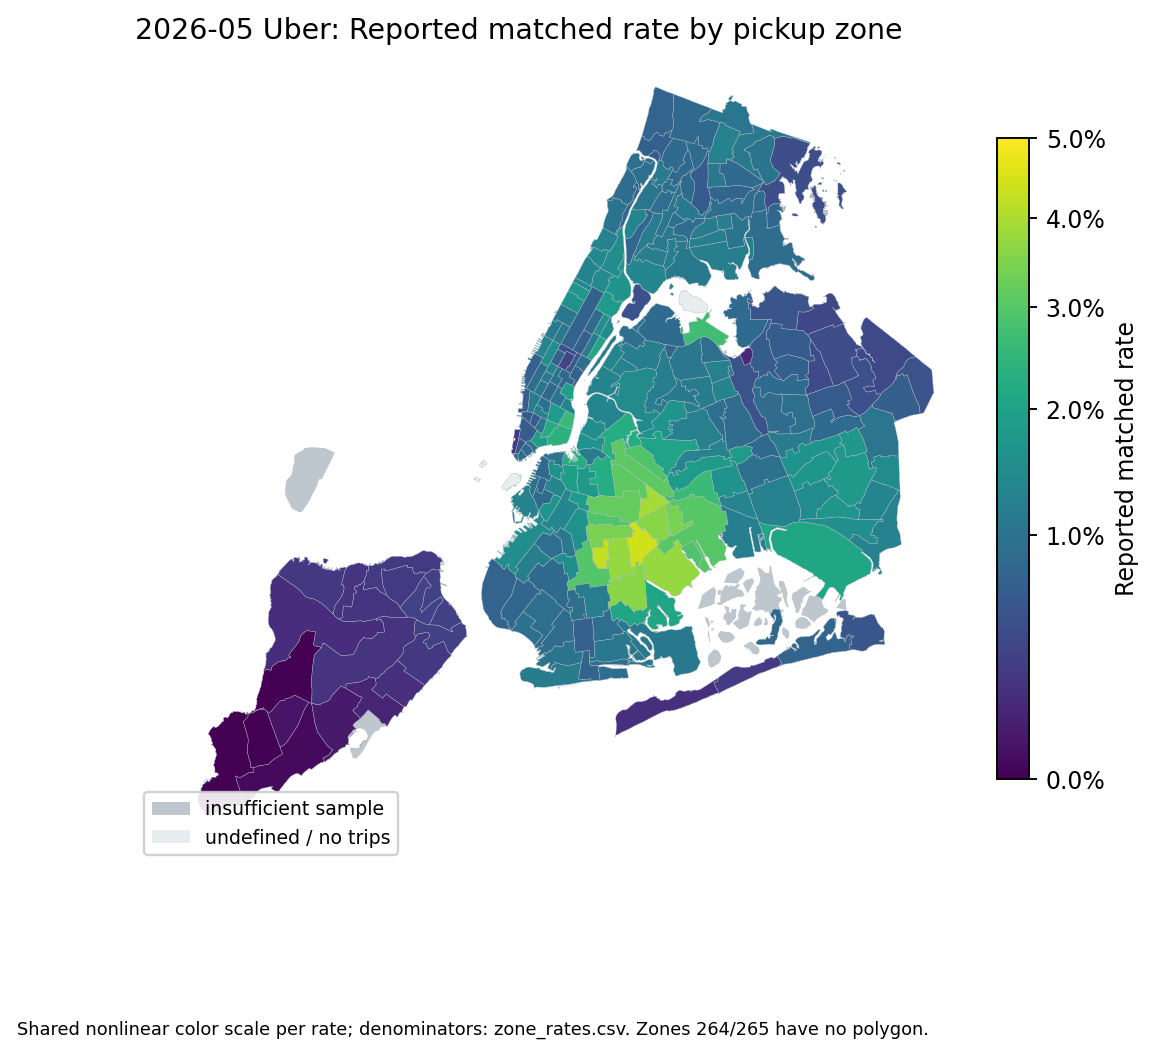
\includegraphics[width=.83\textwidth,height=.72\textheight,keepaspectratio]{04_Results/Task_3/figures/reported_matched_rate_2026-05_uber.png}
\caption{2026-05 Uber reported matched rate by pickup zone, denominator: valid-status trips. Gray zones have fewer than 100 valid-status trips; pale zones have an undefined rate. A gray zone is not a measured zero rate.}\label{fig:share05uM}
\end{figure}

\begin{figure}[p]\centering
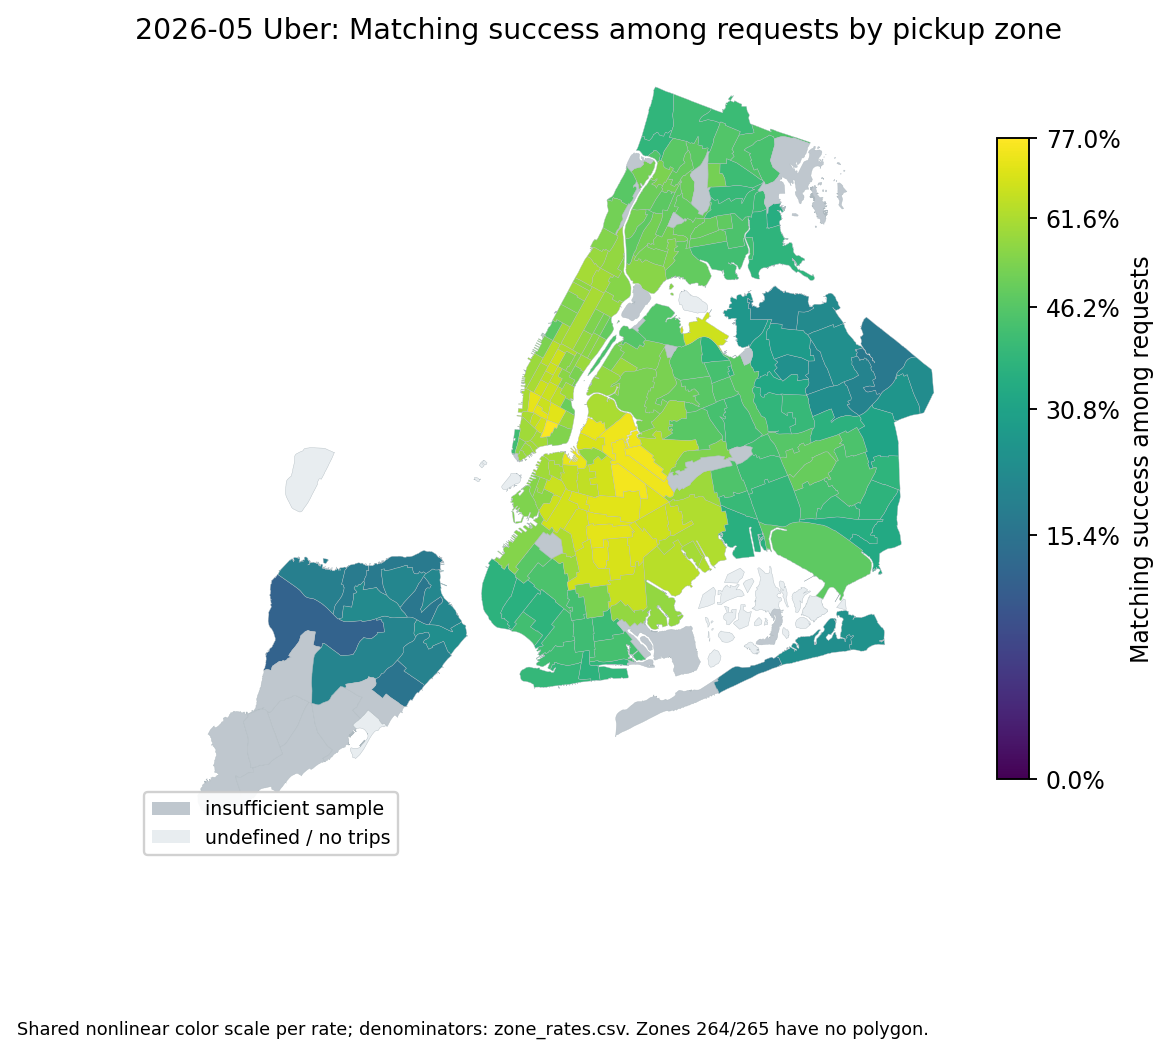
\includegraphics[width=.83\textwidth,height=.72\textheight,keepaspectratio]{04_Results/Task_3/figures/matching_success_2026-05_uber.png}
\caption{2026-05 Uber matching success among pooling requests by pickup zone. Only 233 zones meet the 100-request reporting threshold; gray zones have insufficient requests and pale zones have no defined rate. Colors should be read only for reportable zones.}\label{fig:share05uS}
\end{figure}

\begin{figure}[p]\centering
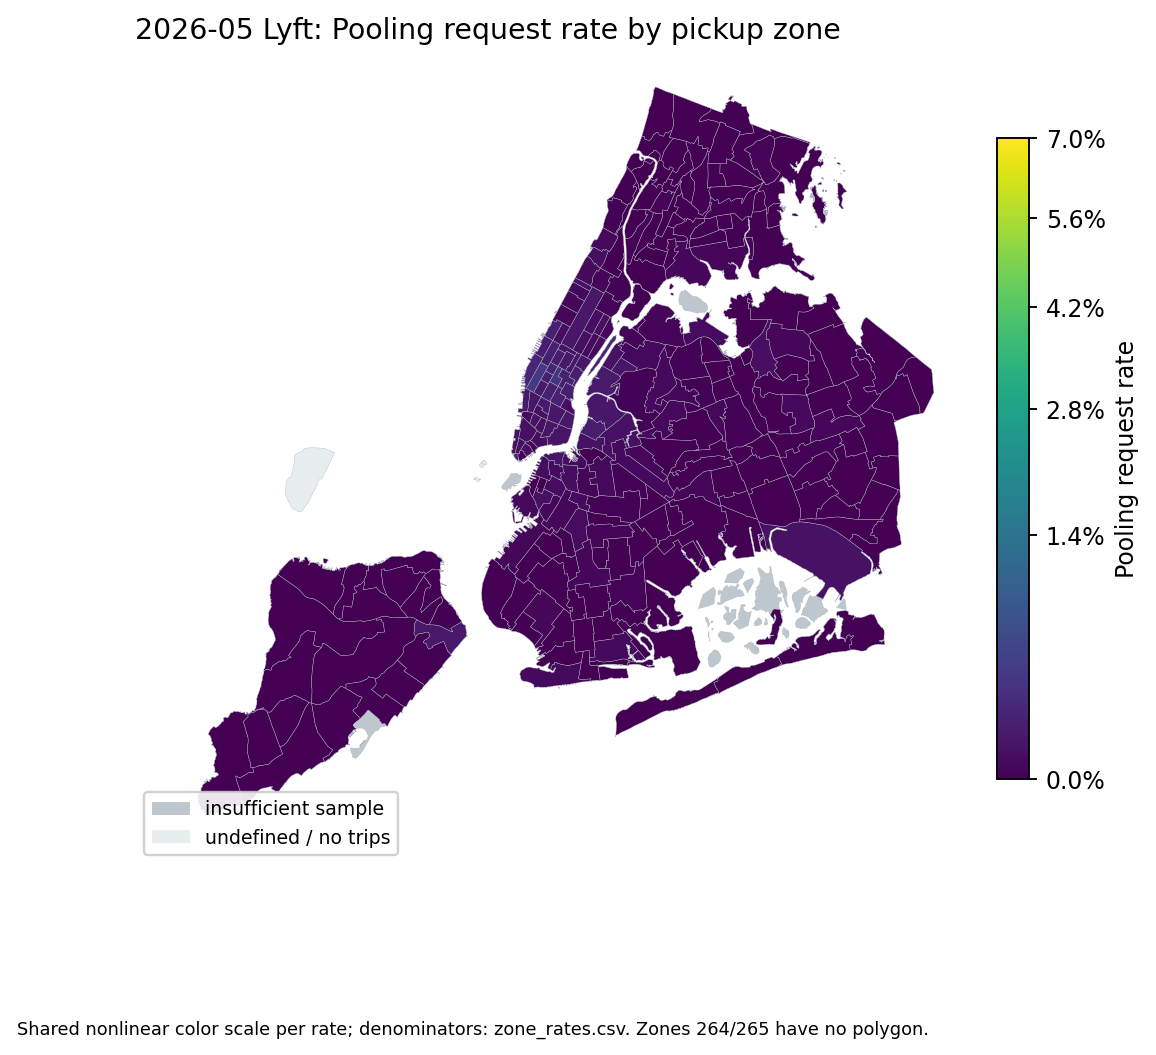
\includegraphics[width=.83\textwidth,height=.72\textheight,keepaspectratio]{04_Results/Task_3/figures/pooling_request_rate_2026-05_lyft.png}
\caption{2026-05 Lyft pooling request rate by pickup zone, denominator: valid-status trips. Gray zones have fewer than 100 valid-status trips; pale zones have an undefined rate. A gray zone is not a measured zero rate.}\label{fig:share05lQ}
\end{figure}

\begin{figure}[p]\centering
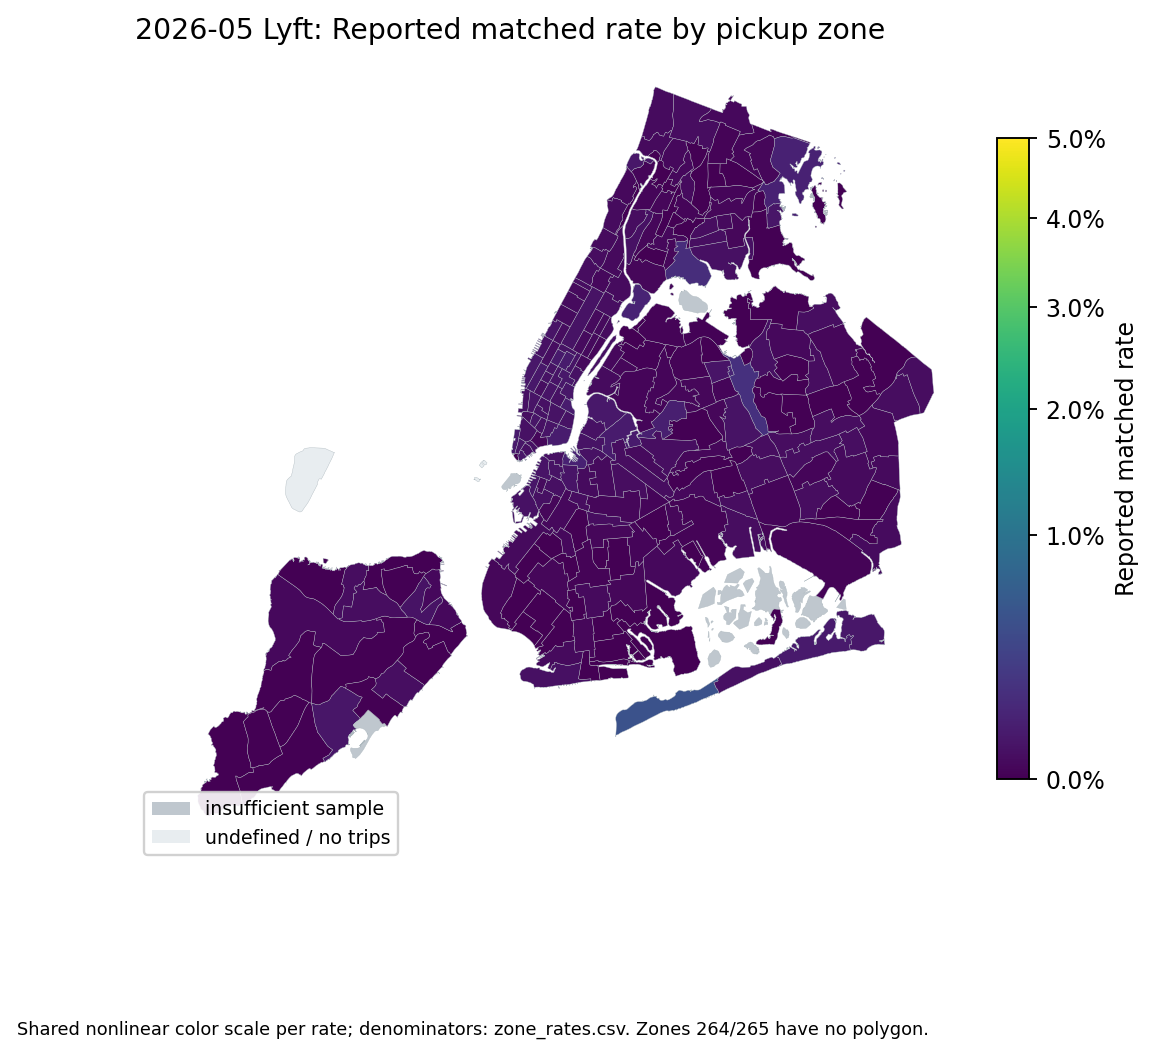
\includegraphics[width=.83\textwidth,height=.72\textheight,keepaspectratio]{04_Results/Task_3/figures/reported_matched_rate_2026-05_lyft.png}
\caption{2026-05 Lyft reported matched rate by pickup zone, denominator: valid-status trips. Gray zones have fewer than 100 valid-status trips; pale zones have an undefined rate. A gray zone is not a measured zero rate.}\label{fig:share05lM}
\end{figure}

\begin{figure}[p]\centering
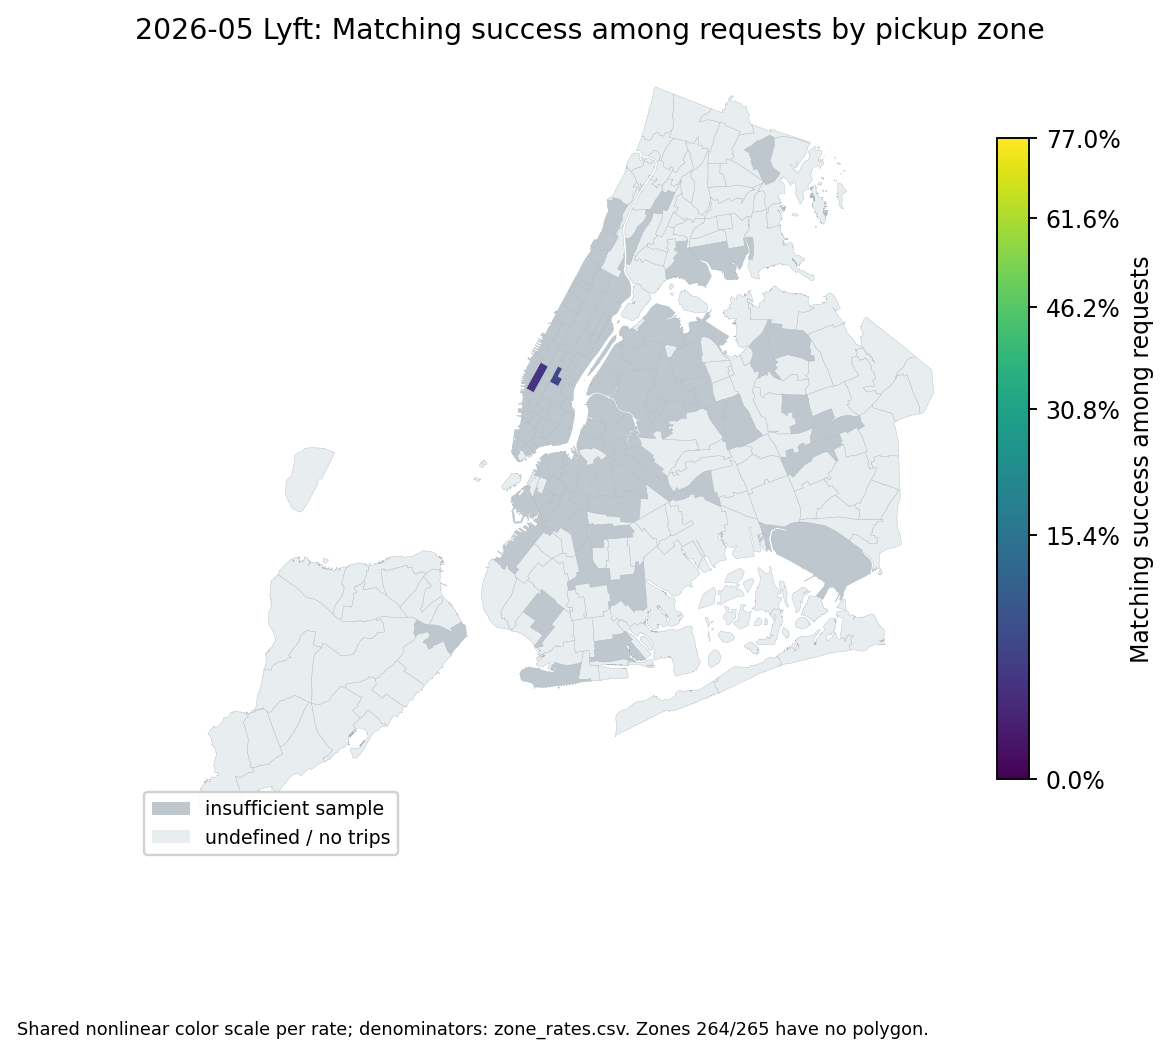
\includegraphics[width=.83\textwidth,height=.72\textheight,keepaspectratio]{04_Results/Task_3/figures/matching_success_2026-05_lyft.png}
\caption{2026-05 Lyft matching success among pooling requests by pickup zone. Only 2 zones meet the 100-request reporting threshold; gray zones have insufficient requests and pale zones have no defined rate. Colors should be read only for reportable zones.}\label{fig:share05lS}
\end{figure}

\clearpage\subsection{Uber excess-time geography}

\begin{figure}[p]\centering
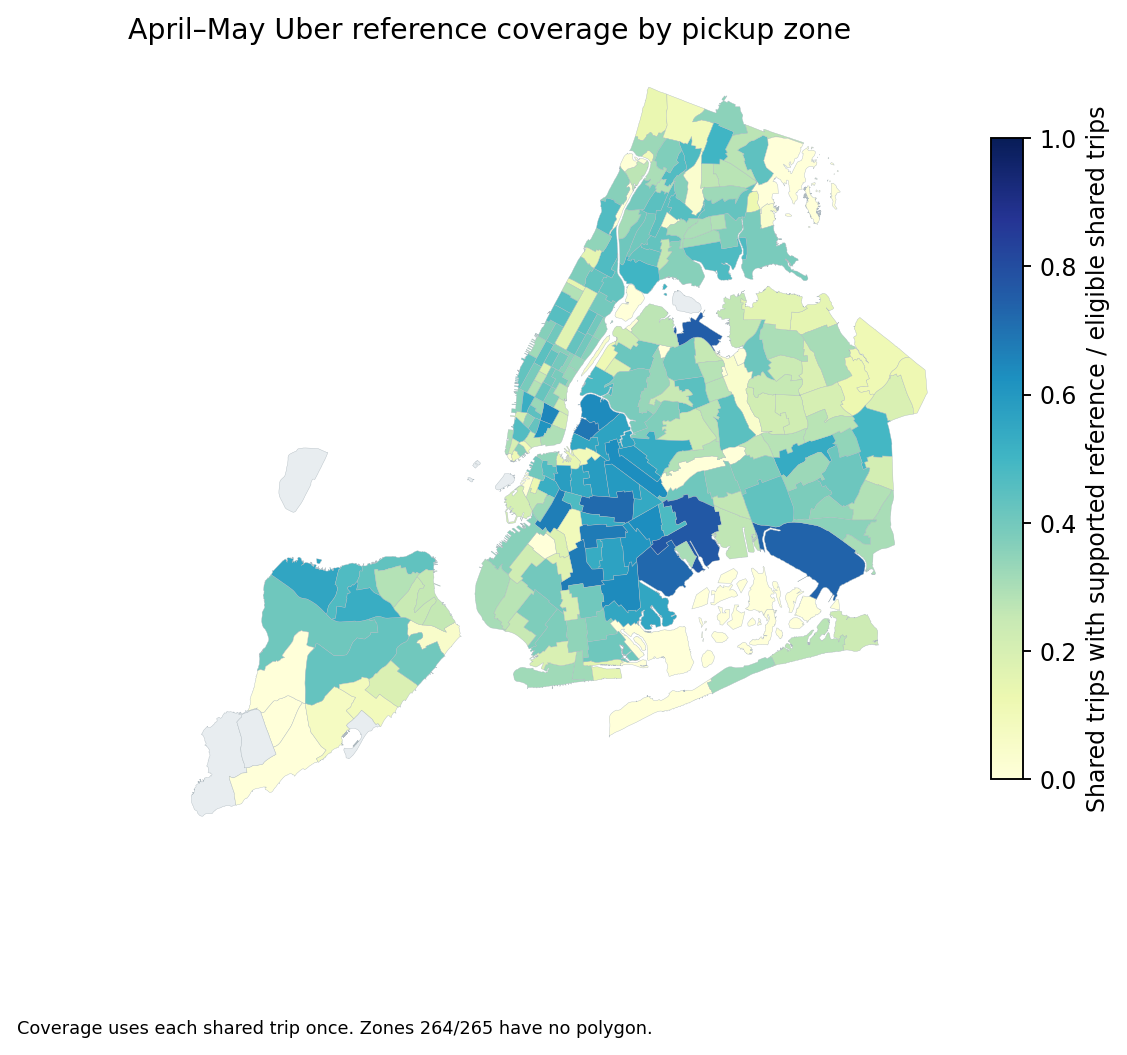
\includegraphics[width=.83\textwidth,height=.72\textheight,keepaspectratio]{04_Results/Task_4/figures/reference_coverage_zone.png}
\caption{Uber Y/Y reference coverage by pickup zone across April--May. Spatially uneven coverage limits interpretation of excess-time maps.}\label{fig:t4coverage}
\end{figure}

\begin{figure}[p]\centering
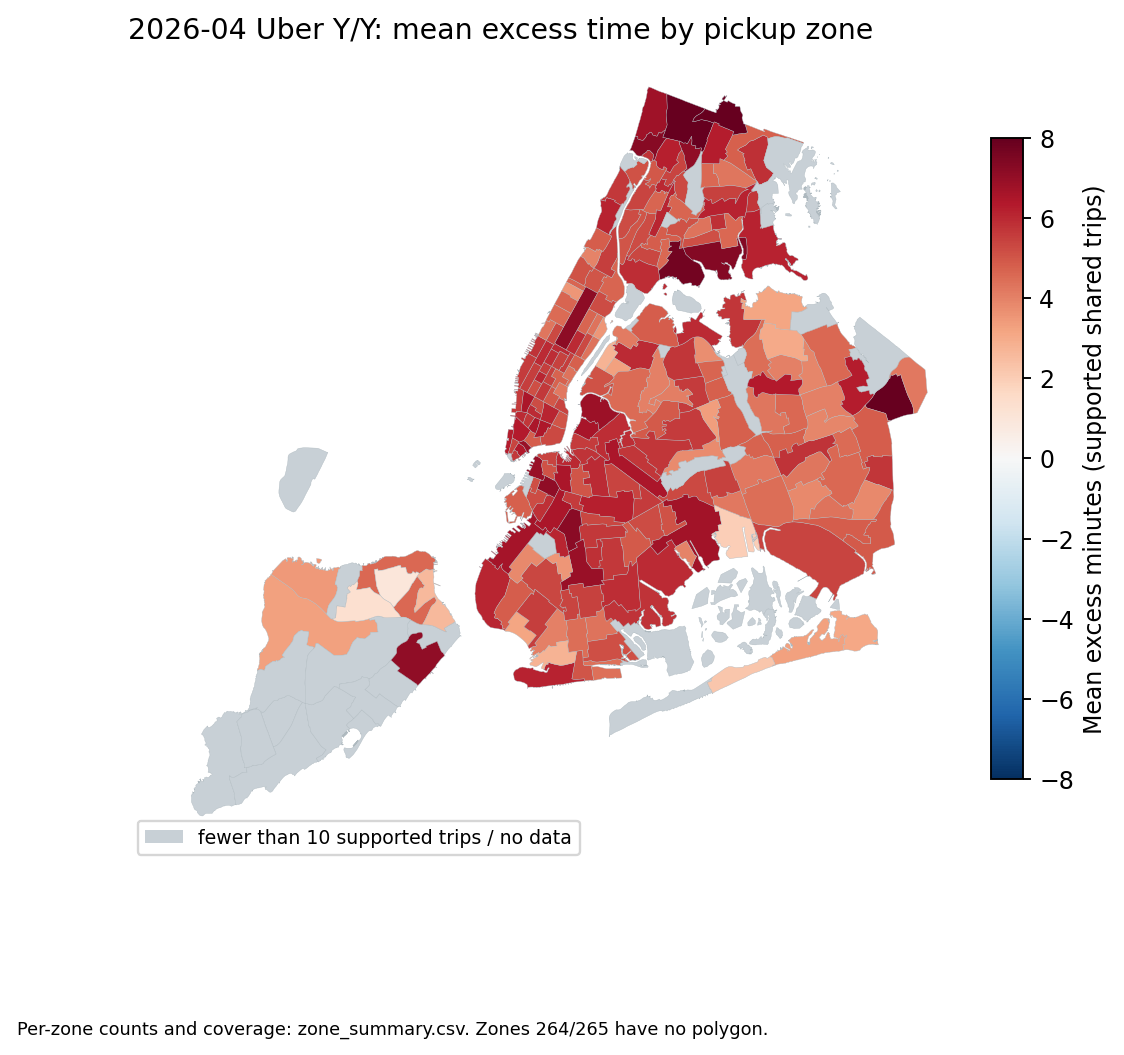
\includegraphics[width=.83\textwidth,height=.72\textheight,keepaspectratio]{04_Results/Task_4/figures/mean_excess_zone_2026-04.png}
\caption{2026-04 mean non-null excess minutes for Uber Y/Y trips by pickup zone. Mapped zones have at least ten supported shared trips; this is an observed difference, not a causal effect.}\label{fig:t4april}
\end{figure}

\begin{figure}[p]\centering
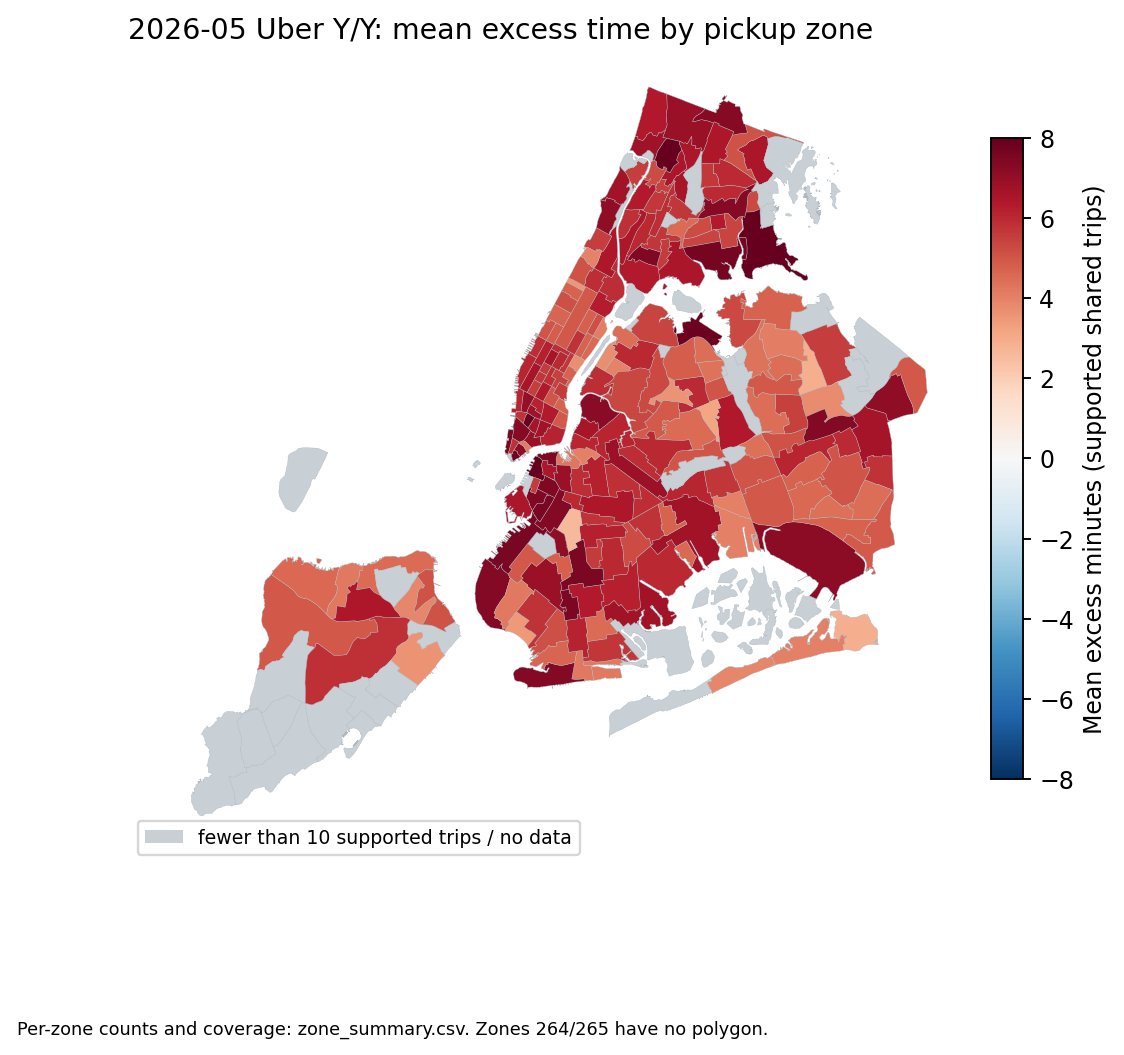
\includegraphics[width=.83\textwidth,height=.72\textheight,keepaspectratio]{04_Results/Task_4/figures/mean_excess_zone_2026-05.png}
\caption{2026-05 mean non-null excess minutes for Uber Y/Y trips by pickup zone. Mapped zones have at least ten supported shared trips; this is an observed difference, not a causal effect.}\label{fig:t4may}
\end{figure}
